\documentclass[a4paper,10pt]{report}
\usepackage[french]{babel}
\usepackage[utf8]{inputenc}
\usepackage[left=2.5cm,top=2cm,right=2.5cm,nohead]{geometry}
\usepackage{url}
\usepackage[T1]{fontenc}
\usepackage{float}
\usepackage{afterpage}
\usepackage{amsmath}
\usepackage{graphicx}
\usepackage{tabularx}
\usepackage{csquotes}
\usepackage{fullpage}
\usepackage{blindtext}
\usepackage[section]{placeins}

\usepackage[toc]{multitoc}
\renewcommand*{\multicolumntoc}{2}
\setlength{\columnseprule}{0.5pt}

\usepackage[pdftex,
            pdfauthor={A. Caccia, A. Madeira Cortes, N. Marchant, R. Fontaine},
            pdftitle={Contrôle automatique d'une serre},
            pdfsubject={Contrôle automatique d'une serre},
            hidelinks,
            pdfcreator={Microsoft Word 1999 Millenium Limited Pro Gold Edition}
            ]{hyperref}

\linespread{1.1}

\setlength{\parskip}{0.5em}

\begin{document}

\begin{titlepage}
    \begin{center}
        \textbf{\textsc{Université Libre de Bruxelles}}\\
        \textbf{\textsc{Faculté des Sciences}}\\
        \textbf{\textsc{Département d'Informatique}}

        \vfill{}
        \vfill{}

        \begin{center}
            {\Huge Contrôle automatique d'une serre}
        \end{center}

        {\Huge \par}

        \begin{center}
            {\large A. Caccia, A. Madeira Cortes, N. Marchant, R. Fontaine}
        \end{center}

        {\Huge \par}
        \vfill{}
        \vfill{}

        \begin{flushleft}
            {\large \textbf{Superviseurs :} M. Labbé, T. Lenaerts}
            \hfill{}
        \end{flushleft}

        {\large\par}
        \vfill{}
        \vfill{}
        % \enlargethispage{3cm} % do not remove

        \textbf{Année académique 2015--2016}
    \end{center}
\end{titlepage}

\renewcommand{\abstractname}{Abstract}
\begin{abstract}

Ce rapport présente différents algorithmes de contrôle automatique et compare leurs performance dans le cas où ils sont utilisés pour contrôler la luminosité d'un système physique régulé en boucle fermée.

Les algorithmes de contrôle étudiés sont Bang bang, PID, ses variantes P et PI ainsi que MPC. Suite au choix d'implémenter les quatre premiers, plusieurs techniques pour améliorer PID on été étudiées et comparées. Ces techniques ont pour but de trouver des paramètres optimaux maximisant la performance de PID.

Pour comparer les performances des algorithmes, nous présentons différentes métriques de scores et nous évaluerons leurs corrélations.

Ces algorithmes ont été implémentés en Python pour être testés et comparés. Ils ont ensuite été utilisés dans des conditions réelles : une serre autonome présentée lors du Printemps des Sciences de l'Université Libre de Bruxelles (Belgique). Celle-ci utilisait les algorithmes de contrôle présentés ci-dessus pour gérer la température, la luminosité et l'humidité du sol et les stabiliser au plus près de leurs valeurs idéales pour les plantes s'y trouvant.

Cette étude montrera l'efficacité de PID pour le contrôle de phénomènes spontanés, telles que la gestion de l'intensité de la lumière, tout en soulignant la suffisance de Bang Bang pour des contrôles plus simples, comme le contrôle de la température.
Elle démontrera également les avantages et inconvénients des méthodes de détermination des paramètres de PID.
\end{abstract}

\tableofcontents

\chapter{Introduction}

Au vu de la pollution grimpant de façon astronomique dans les grandes villes et mégalopoles, de nombreuses méthodes pour baisser les émissions de gaz à effet de serre ont été créées depuis quelques années. L'une d'elles est de construire des serres dans les toits ou caves inutilisées d'immeubles. L'entretien et la maintenance de ces serres étant relativement coûteuse en moyens humains, il est intéressant de pouvoir automatiser une partie du travail.

Le fait de faire pousser de la nourriture localement dans les grandes villes a pour grand avantage de réduire considérablement le nombre de camions entrant et sortant de la ville pour effectuer des livraisons. De plus, dans certains cas, le rendement est jusqu'à 100 fois plus grand pour une même surface pour 40\% moins d'énergie consommée, 40\% moins de pertes d'aliments et 99\% moins d'utilisation d'eau que la production traditionnelle. \cite{GEReports}

Nous avons donc choisi comme projet pour le Printemps des Sciences de l'Université Libre de Bruxelles de fabriquer une serre qui régule la température, l'humidité du sol et la luminosité de manière autonome. Lors de cet évènement, deux dispositifs pédagogiques ont été crées pour expliquer le projet aux visiteurs: Le premier était une serre contenant des plantes, dans laquelle les variables citées plus haut étaient régulées en direct. Le deuxième dispositif était une boite en plastique, modifiée pour accommoder un capteur de température, des ventilateurs et un sèche cheveux, utilisée pour démonter la régulation de la température sans perturber les plantes se trouvant dans la serre.

Pour construire une telle serre, il est nécessaire d'étudier en détail le matériel requis pour l'automatiser, notamment les capteurs et l'électronique à créer pour mesurer et agir sur l'environnement de la serre en temps quasi réel.
Il est aussi important d'étudier et analyser un type d'algorithmes dits de ``contrôle'', qui nous permettraient de créer l'aspect automatisé de la serre.

Dans la serre, l'algorithme PID était appliqué, tandis que dans la boite en plastique il s'agissait de Bang Bang. Les visiteurs pouvaient voir les données mesurées sur un écran, et donc voir en temps réel lorsque le système subissait une perturbation (et la correction qui était appliquée).

\chapter{État de l'art}

Cet état de l'art est séparé en deux parties : la première détaille les différentes méthodes de régulation automatique et la seconde étudie les différentes méthodes pour configurer l'algorithme \emph{PID}, détaillé en \ref{PID}.

\section{Contrôle automatique}
L’automatique est une science qui étudie la modélisation, l’analyse et la commande de systèmes dynamiques.
L’automatique permet de contrôler un système en respectant un cahier des charges (rapidité, précision, stabilité, ...).

L'automatique était un sujet assez vaste, nous nous limiterons ici à l'étude des différentes méthodes de contrôle permettant de stabiliser l'état d'un système au plus proche d'une valeur consigne.

Nous étudierons premièrement \emph{BangBang}, l'algorithme le plus simpliste, utilisé dans les thermostats.
Ensuite nous étudierons \emph{PID} ainsi que ses variantes.
Pour finir nous survolerons \emph{MPC}, un algorithme prédictif plus avancé.

\subsection{\emph{Bang bang}}
Le \emph{``Bang bang control''} aussi appelé \emph{``On-Off control''} ou en français \emph{``Tout ou rien''} est un contrôleur qui ne peut accepter que deux états de contrôle tels que ouvert ou fermé, allumé ou éteint.

Des exemples très classiques d'utilisation de ce type de contrôleur sont les thermostats: le chauffage s'allume sous une température minimale, et s'éteint au-dessus d'un seuil maximal.

Nonobstant la facilité d'implémentation et de mise en place de cet algorithme, son utilisation ne peut être généralisée au contrôle de phénomènes spontanés. En effet, si l'on prend l'exemple du contrôle de la luminosité, \emph{bang bang} ne pourra qu'allumer ou éteindre des lampes, il ne pourra influer sur leur intensité. \cite{Burghes2004}

De plus, cet algorithme ne permet pas une stabilité suffisante : en effet, une fois la correction atteinte, \emph{Bang bang} n'agira plus jusqu'à ce que les perturbations soient trop importantes et cela produira une oscillation permanente. \cite{ballard1993pid}


\subsection{\emph{PID}}
\label{PID}

\emph{PID} est le régulateur le plus connu et le plus utilisé dans le domaine industriel : il serait utilisé dans plus de 95\% des systèmes \cite{Kinnaert2013, aastrom2002control}.
Il porte ce nom à cause de son fonctionnement qui est découpé en trois actions : l'action proportionnelle, l'action intégrale et l'action dérivée.

PID est défini par la fonction suivante:

\begin{equation}
  u(t) =
    \underbrace{K_p e(t)}_{P} +
    \underbrace{K_i \int_{0}^{t} e(\tau) d\tau}_{I} +
    \underbrace{K_d \frac{de}{dt}.}_{D}
\end{equation}

Dans laquelle $u(t)$ est la sortie de PID qui doit être appliquée à l'élément à contrôler et P, I et D sont les trois composantes ci-dessous :
\begin{description}
\item[Action proportionnelle (P) :]
    est proportionnelle à l'erreur de contrôle courante.
\item[Action intégrale (I) :]
    fait varier la réponse de PID en fonction des valeurs passées de l'erreur de contrôle.
\item[Action dérivée (D) :]
    est basée sur les valeurs futures estimées pour l'erreur de contrôle.
\end{description}

Les premières analyses techniques de \emph{PID} datent de 1922, lorsque Nicolas Minorsky essaye de créer des systèmes de pilotage automatique pour la marine des États-Unis. \cite{minorsky1922directional}

Malgré le fait que de nombreuses autres techniques ont été inventées depuis la création de \emph{PID}, il maintient son fonctionnement de base et a simplement évolué avec le temps et sert parfois de composant de base à d'autres contrôleurs plus complexes \cite{ang2005pid} \cite{visioli2006practical}

Il maintient sa popularité car il est souvent admis qu'aucun autre contrôleur n'égale la simplicité, le fonctionnement clair, la facilité d'application et d'utilisation offerte par \emph{PID}. Cette facilité d'utilisation vient du fait qu'il se base uniquement sur des variables mesurées, sans connaissance du procédé sous-jacent et qu'il a donc énormément d'applications différentes \cite{bennett1993history}.

Il est aussi possible dans quelques applications de PID que certaines actions soient inutiles.
Dans ce cas-là, on parle de contrôleurs PI, PD, P ou I.
Par exemple, une des raisons d'enlever l'action dérivée est qu'elle est fort sensible au bruit lors des mesures \cite{svrcek2014real}.

\subsection{P controller}
Le \emph{Proportional Control} est l'ancêtre du PID, il ne prend en compte que la partie proportionnelle de celui-ci.
Cet algorithme se situe entre l'algorithme Bang Bang et PID:
en effet, là où \emph{Bang Bang} va corriger l'état simplement en allumant ou en éteignant un appareil, l'algorithme P control va lui, appliquer une réponse appropriée à la perturbation.

Un tel contrôleur s'exprime par l'équation
\begin{equation}P_{out} = K_{P}e(t) + p_0\end{equation}
dans laquelle $e(t)$ est l'erreur (la différence entre valeur attendue et valeur mesurée), $K_{P}$ est le paramètre de gain proportionnel, $P_{out}$ est la réponse à la perturbation et $p_0$ est la correction à appliquer, nécessaire vu que cet algorithme n'a pas de composante intégrale (contrairement à PID).

Un grand avantage de l'utilisation de ce type de contrôleur est qu'il n'y a qu'un seul paramètre à configurer, qui définit à quel point la correction sera agressive : plus le paramètre $K_{p}$ est petit (respectivement grand), plus la réaction est lente (respectivement rapide).

Si l'implémentation d'un tel contrôleur est aisée, ses sorties produisent un phénomène d'\emph{offset} : un décalage par rapport aux valeurs attendues \cite{svrcek2014real}.

Le choix d'un tel contrôleur par rapport à PID dépend de l'utilisation, de la précision et de la vitesse des corrections désirées.
Des exemples où l'algorithme P control est suffisant sont donnés dans \cite{sellers2001overview}.

\subsection{\emph{Integral controller}}
Le principe d'un \emph{Integral controller} est de corriger un offset résultant de l'utilisation d'un P controller.
Un tel contrôleur est caractérisé dans \cite{svrcek2014real} par l'équation
\begin{equation}P_{out} = \frac{1}{T_{i}}\int e dt + MV_{0}\end{equation}
où $MV_{0}$ correspond à la correction biaisée de P controller,
$\int e dt$ représente l'intégrale des erreurs sur l'intervalle de temps $dt$ et $T_{i}$ est le temps intégral défini comme le temps nécessaire pour changer la sortie du contrôleur d'une quantité égale à l'erreur.

Bien que ce contrôleur propose une correction aux décalages, on observe un temps de réponse jusqu'à dix fois inférieur inférieur à l'utilisation d'un P controller seul \cite{svrcek2014real}.

\subsection{PI controller}
Un contrôleur PI utilise à la fois l'action proportionnelle et l'action intégrale.
Il est caractérisé par l'équation
\begin{equation}P_{out} = K_{P} e + K_{I} \int e dt\end{equation}
où $K_{p}$ et $K_{I}$ sont les paramètres de réglages proportionnel et intégral
et les autres symboles correspondent à ce qui est indiqué dans les sections \emph{P controller} et \emph{Integral controller}.

Ces contrôleurs sont 50\% plus lents qu'un contrôleur P seul, mais plus rapides que l'ajout d'un contrôleur intégral séparé \cite{svrcek2014real}.
En effet, si l'on compare son équation avec celle du P controller, le terme $p_0$ a été remplacé par une correction intégrale, ce qui corrige l'erreur automatiquement.

\subsection{MPC controller}
\emph{MPC} est un contrôleur permettant la régulation de différentes variables dans un système.
Celui-ci utilise à la fois des stratégies prédictives et l'état actuel afin de calculer les prochaines états possibles \cite{RICHALET1978413}.

Contrairement à PID, MPC accepte des systèmes ayant de multiples valeurs d'entrées et devant sortir également plusieurs valeurs.
Par contre, de nombreux modèles MPC ne supportent que les circuits en boucle ouverte.
Il demande également plus de ressources à la fois logicielles et matérielles \cite{saletovic2014apm}.
De plus, ils nécessitent un grand nombre de modèles pour interpoler la réponse et si la commande prédictive est erronée, les performances vont être faibles même si les modèles sont corrects \cite{Richalet2016}.

Une comparaison entre APM (une variante simple de MPC) et PID a été faite dans \cite{saletovic2014apm}, et montre qu'avec des configurations optimales, APM a apporté un meilleur contrôle que PID, mais PID a requis moins de ressources et possède un temps de stabilisation plus court.

\section{Détermination des paramètres de PID}

\emph{PID} étant inefficace et donc inutile si ses paramètres (les constantes $K_p$, $K_i$, $K_d$) sont mal fixés, il nous semble important d'aussi étudier les différentes méthodes pour les déterminer. Il existe énormément de méthodes différentes pour configurer \emph{PID}.

Les effets (positifs ou négatifs) de l'ajustement des paramètres sont, entre autres \cite{zhong2006pid} :
\begin{enumerate}
\item la stabilité (la tendance à rester dans un interval de valeurs),
\item la précision (la tendance à rester autour de la consigne),
\item la rapidité (le temps d'attente avant que le système n'arrive à la stabilité)
\end{enumerate}

Nous étudierons ici trois méthodes manuelles ainsi que deux méthodes heuristiques.

Nous encourageons le lecteur à se référer à \cite{shahrokhi2013comparison} qui fait une revue plus détaillée et complète des différentes méthodes pour déterminer les paramètres.


\subsection{La méthode manuelle}

La méthode manuelle est une technique où un opérateur humain modifie les paramètres manuellement, sans algorithme déterminé, jusqu'à obtenir un résultat satisfaisant. Cette technique s'applique sur un système en fonctionnement.

L'avantage de cette technique est qu'elle ne nécessite aucun calcul mathématique complexe. Cependant, elle requiert l'interaction d'un technicien expérimenté, étant donné que chaque variation des paramètres implique de très nombreuses modifications sur le résultat obtenu (croissance initiale, stabilité, délai d'attente jusqu'à la stabilité, dépassement, ...). \cite{zhong2006pid}


\subsection{Ziegler–Nichols}
% ziegler1942optimum
% silva2007pid
% http://www.chem.mtu.edu/~tbco/cm416/tuning_methods.pdf
Comme la méthode manuelle, Ziegler–Nichols s'applique aussi sur un système en fonctionnement. Cependant, elle utilise des calculs un peu plus complexes que la méthode manuelle mais son avantage est qu'elle nécessite des techniciens moins expérimentés.\cite{ziegler1942optimum}
En effet, cette méthode requiert peu d'informations sur le système en fonctionnement, étant donné que les formules utilisées découlent d'un nombre exhaustif de simulations de systèmes stables et simples. \cite{silva2007pid}

Une des critiques qui peut être faite à cette méthode est que dans la plupart du temps elle donne des bons résultats mais dans certains cas le résultat est fort erroné,
menant à un mauvaise stabilité et un faible amortissement des perturbations.

De plus, cette méthode produit systématiquement un dépassement lors de la montée initiale et
puis se met à osciller avec une amplitude d'oscillation qui décroit linéairement au cours du temps.
Elle n'est donc pas utilisable dans tout les système
 et est particulièrement déconseillée lorsque le système ne peut pas dépasser fortement la valeur cible \cite{silva2007pid}.

\subsection{Recherche Tabou}

Il est aussi possible de déterminer des paramètres pour PID à l'aide la méthode de la recherche Tabou.

La recherche Tabou est une méthode heuristique d'optimisation utilisée quand l'expression analytique de la fonction à minimiser n'est pas connue
(comme dans le cas de PID si le système à stabiliser n'a pas été modélisé mathématiquement ou physiquement).

La recherche Tabou est une recherche locale qui part d'un point arbitraire et compare ses points proches afin de tenter de trouver le minima de celle-ci.
Le mot Tabou vient du fait qu'il faut pas tomber dans un minima local et y rester :
cet algorithme garde donc une liste des minimas locaux, la liste des tabous, pour ne pas y retomber.

Une comparaison entre résultats obtenus avec la méthode de Ziegler-Nichols et la recherche Tabou se trouve dans \cite{Karaboga569754}.
Une autre implémentation citée dans \cite{bagis2011tabu} compare la recherche Tabou avec plusieurs autres algorithmes et démontre l'efficacité de la méthode.

\subsection{Algorithmes génétiques}

Les algorithmes génétiques sont un type d'algorithme évolutif qui mimique la théorie de l'évolution afin de raffiner des résultats par un procédé itératif aléatoire, ce qui en fait une méthode méta-heuristique.

Plusieurs avantages et inconvénients sont discutés dans \cite{Tabassum2014}.
Ces algorithmes permettent l'optimisation d'une large variété de problèmes et sont efficaces pour déterminer plusieurs paramètres à la fois.
Cependant, ces algorithmes nécessitent une grande population et beaucoup de générations pour converger vers un bon résultat, ce qui peut rendre les temps d'exécutions assez élevés.
De plus, un mauvais choix de la fonction de score (voir \ref{section:metrics}) pourra conduire à un résultat médiocre voir tout à fait faux qui ne sera remarqué qu'à la fin de l'exécution de l'algorithme.

Une comparaison des performances obtenues entre un PID paramétré via la méthode de Ziegler-Nichols et via un algorithme génétique est disponible dans \cite{thomas2009position} et a montré un temps de réponse bien meilleur pour l'algorithme génétique.

\chapter{Implémentation}
\label{chap:impl}

L'implémentation de ce projet a été découpé en trois phases : premièrement nous avons construit un prototype physique d'un serre et de son système de contrôle (capteurs, lumières, ...); ensuite nous avons implémenté en software un protocole de communication ainsi qu'un driver pour communiquer avec le hardware et le contrôler; pour finir, nous avons implémenté en Python différents algorithmes de contrôle.

\section{Implémentation hardware et firmware}

La partie hardware de ce projet qui a été utilisée pour l'étude de l'efficacité des algorithmes de contrôle est composée d'un Arduino connecté à une photo-résistance ainsi qu'à un transistor de puissance qui contrôle de puissantes LED.

La luminosité ambiante est mesurée grâce aux variations de résistance du capteur de luminosité qui, mise en valeur par notre circuit, est mesurée comme un changement de tension aux bornes du convertisseur digital-analogique de l'Arduino.

La puissance d'éclairage, quant à elle est contrôlée par des pulsations plus ou moins espacées (en fonction de la puissance demandée) envoyées en 5 volts par une des sorties de l'Arduino et qui sont ensuite amplifiées en 12 volts par le transistor de puissance.

Ensuite, nous avons mis en place un protocole de communication via le port série de l'Arduino pour permettre à un PC de lui envoyer des ordres (par exemple : ``allumer la LED 2 à 55\%'') ainsi que de récupérer la valeur des capteurs (par exemple ``récupérer la résistance de la photo-résistance 4''). Cette interface de communication a ensuite été adaptée pour être utilisable facilement en Python depuis une librairie intuitive utilisable dans la partie suivante.


\section{Implémentation software}

Nous avons décidé d'implémenter \textit{Bang-bang} et \textit{PID} ainsi que différentes méthodes pour déterminer les paramètres de \textit{PID} afin de pouvoir les comparer par la suite.

Ces implémentations ont été réalisées dans le langage de programmation Python, afin de tirer parti de sa rapidité de développement et ses librairies de calcul scientifique, telles que Numpy et Scipy.

\subsection{Contrôle automatique}
\label{sec:contr-implem}
Le contrôle automatique étant dominé par la combinaison de \textit{Bang-bang} et \textit{PID}, nous avons choisi d'étudier en détail ces deux-ci ainsi que les variantes \textit{P} et \textit{PI}.

\subsubsection{\emph{Bang-bang}}

L'implémentation de \emph{Bang-bang} est simple: une fonction reçoit en paramètre la variable à contrôler et observe si celle-ci est en-dessous (respectivement au-dessus) d'un seuil dans le cas où la correction tend à augmenter (respectivement diminuer) la variable. Elle renvoie ensuite en conséquence un état: allumé ou éteint.

L'implémentation que nous avons écrite fonctionne simplement : à chaque fois que la fonction de contrôle est appelée, elle regarde si l'entrée est trop basse et si oui, la sortie est l'état activé, si non, l'état désactivé.

\subsubsection{PID}

\emph{PID} tentant de minimiser l'erreur au long du temps en s'ajustant peu à peu, son implémentation est un peu plus complexe : à chaque appel à la fonction de contrôle, l'erreur courante ainsi que le temps sont enregistrés.
Il est ensuite possible de calculer l'intégrale des erreurs du passé ainsi que la dérivé de l'erreur à l'instant présent.
Nous pouvons donc utiliser ces différentes valeurs pour les introduire dans la formule de PID et les pondérer à l'aide des paramètres ($K_p$, $K_i$ et $K_d$) qui ont été spécifiés pour l'instance du contrôleur et la sortie de cette formule nous donnera la correction à appliquer.

De plus, quand la correction à appliquer dépasse la valeur maximale de ce que le composant physique peut accepter, pour éviter qu'une erreur qui n'est pas complètement corrigeable à cause de limitations physiques ne pénalise trop la partie intégrale dans le futur, nous tronquons la valeur ajoutée à cette intégrale à la limite physique. Par exemple, on ne peut demander à une ampoule allumée à fond de briller plus.

\subsection{Détermination des paramètres de PID}

Nous avons implémenté plusieurs méthodes pour déterminer des bons paramètres pour PID. Celles-ci vont de la méthode manuelle qui ne nécessite pas de code et uniquement quelques calculs aux algorithmes génétiques qui nécessitent plusieurs dizaines d'heures de simulation.

\subsubsection{La méthode manuelle}

Cette méthode est effectuée à la main par un technicien expérimenté.
L'algorithme se déroule en 4 étapes:
\begin{enumerate}
    \item Les valeurs des 3 paramètres sont fixées à $0$.
    \item Le paramètre $K_p$ est incrémenté jusqu'à ce que la sortie du système se mette à osciller.
    On prendra comme valeur pour $K_p$ la moitié de celle obtenue précédemment.
    \item $K_i$ est augmenté jusqu'au moment où l'offset est corrigé dans un temps acceptable pour le système.
    \item Si nécessaire, $K_d$ est augmenté jusqu'au moment où la boucle est suffisamment rapide pour atteindre à nouveau la consigne après une perturbation extérieure.
\end{enumerate}

\subsubsection{Ziegler–Nichols}
La méthode de Ziegler–Nichols quant à elle peut soit être effectuée à la main soit avec l'aide d'un ordinateur qui effectue les calculs ou de manière autonome, si on implémente un algorithme de détection d'oscillations.

Elle fonctionne comme ceci :
\begin{enumerate}
    \item Les valeurs des 3 paramètres sont fixées à $0$.
    \item $K_p$ est augmenté jusqu'à ce que la sortie de la boucle oscille (cette détection peut être manuelle ou automatique).
\end{enumerate}

Une fois que l'oscillation est détectée, la valeur de $K_p$ ainsi obtenue est gardée et nommée $K_u$ ainsi que la période de l'oscillation : $P_u$.
Ensuite, les autres paramètres sont déterminés à l'aide du tableau \ref{tab:ZieglerNicholsTuningFormulas}

\def\tabularxcolumn#1{m{#1}}
\begin{figure}[ht]
    \begin{center}
        \begin{tabularx}{\textwidth}{| c | X | X | X |}
            \hline
            & $K_p$ & $K_i$ & $K_d$\\ \hline
            P & \begin{equation*}\frac{K_u}{2}\end{equation*} & &\\ \hline
            PI & \begin{equation*}\frac{K_u}{2,2}\end{equation*} & \begin{equation*}1,2 \cdot \frac{K_p}{P_u}\end{equation*} &\\ \hline
            PID & \begin{equation*}\frac{K_u}{1,7}\end{equation*} & \begin{equation*}2 \cdot \frac{K_p}{P_u}\end{equation*} & \begin{equation*}K_p \cdot \frac{P_u}{8}\end{equation*} \\
            \hline
        \end{tabularx}
    \end{center}
    \caption{Tableau des formules pour Ziegler–Nichols}
    \label{tab:ZieglerNicholsTuningFormulas}
\end{figure}

\subsubsection{Algorithmes génétiques}
Il est également possible de déterminer ces paramètres à l'aide de ce que l'on appelle un algorithme génétique.
Le principe est de générer aléatoirement une population de chromosomes qui possèdent dans notre cas 3 emplacements (ou \textit{loci}) représentant chacun l'un des paramètres $K_p$, $K_i$ ou $K_d$ à déterminer.

Chaque chromosome est ensuite alors testé: un algorithme PID sera exécuté par chromosome en spécifiant les paramètres de celui-ci et recevra ensuite un score indiquant ses performances (voir \ref{section:metrics}).

En fonction de ce score, les chromosomes auront plus ou moins de chance d'être choisis et procréer: une nouvelle génération va être créée qui contiendra le même nombre de chromosome que la précédente.

Pour ce faire nous appliquons l'algorithme suivant :
\begin{enumerate}
  \item Deux chromosomes sont choisis selon une \textit{roulette wheel selection} : les chromosomes sont choisis aléatoirement, mais avec des probabilités plus importantes selon la grandeur de leur score;
  \item Lors de la reproduction, il y a une forte chance (dans notre cas, 90\%) que le chromosome enfant soit un clone de l'un de ses parents. Si ce n'est pas le cas, il se produit un \textit{crossing-over} : pour chaque \textit{loci} a une chance sur deux de venir du père et une chance sur deux de venir de la mère.
  \item Le chromosome enfant aura ensuite une faible probabilité de subir une ``mutation'': l'un de ses trois paramètres sera remplacé par une valeur aléatoire.
\end{enumerate}

La nouvelle population créée va recommencer le cycle précédent et régénérer une autre population et ainsi de suite un nombre arbitraire de fois.
Une fois ce cycle fini le meilleur chromosome sera sélectionné en fonction de son score et ses paramètres pourront être utilisés par PID.


\chapter{Résultats et discussion}
\label{chap:res}

Après avoir implémenté les algorithmes présentés ci-dessus, nous les avons comparés grâce à un dispositif expérimental que nous avons créé.

\section{Méthode expérimentale}
\label{sec:methode}
Nous avons fabriqué une boite opaque dans laquelle se trouve un capteur de lumière ainsi que deux LEDs de puissance. Le capteur ainsi que la première LED sont reliés à un Arduino\footnote{Un Arduino est un micro-contrôleur programmable en c++ est qui peut communiquer avec un ordinateur par une liaison série} qui fait suivre la valeur du capteur à un programme Python que nous avons écrit et qui récupère la valeur de sortie de ce programme pour contrôler la puissance de la LED.

La seconde LED est utilisée pour perturber le système et ainsi pouvoir mesurer la résistance aux perturbations de nos algorithmes.

Pour comparer deux techniques entre elles, nous lançons 5 simulations à la suite l'une de l'autre pour chacune d'elles.
Et nous attribuons un score à chaque simulation selon les métriques définies en \ref{section:metrics} et le score final d'une méthode est défini comme la moyenne des scores des différentes simulations.

Une simulation consiste en :
\begin{itemize}
    \item Le système est remis à zéro : toutes les lampes sont éteintes et le capteur indique 0 lux.
    \item L'algorithme de contrôle est lancé avec comme consigne de stabiliser le système à 500 lux.
    \item Après 10 secondes, la seconde LED est allumée pour perturber le système
    \item 10 secondes après l'allumage de la seconde LED, la simulation est arrêtée.
    \item Un score est assigné à la simulation en fonction de sa performance.
    \\
\end{itemize}

\label{section:metrics}
Pour nous permettre de comparer les différentes méthodes, nous devons introduire des métriques permettant d'attribuer un score à ces méthodes.
Nous utiliserons ici les métriques utilisées par \cite{griffin2003line, mirzal2012pid} :
\begin{description}
    \item[MSE] : La moyenne de l'erreur au carré (Mean of the Squared Error)
    \item[ITAE] : L'intégrale du temps multipliée par la valeur absolue de l'erreur  (Integral of Time multiplied by Absolute Error)
    \item[IAE] : L'intégrale de la valeur absolue de la magnitude de l'erreur (Integral of Absolute Magnitude of the Error)
    \item[ISE] : L'intégrale de l'erreur au carré (Integral of the Squared Error)
    \item[ITSE] : L'intégrale du temps multipliée par l'erreur au carré (Integral of Time multiplied by the Squared Error)
\end{description}

$$
\textbf{MSE} = \frac{1}{T} \int_0^T e(t)^2 dt,
\textbf{ITAE} = \int t \cdot |e(t)| dt,
\textbf{IAE} = \int |e(t)| dt,
\textbf{ISE} = \int e(t)^2 dt,
\textbf{ITSE} = \int t \cdot e(t)^2 dt
$$

\section{Résultats}

\subsection{Métriques de score}

Pour commencer, nous avons comparé les différentes fonctions de score afin de choisir avec laquelle nous allions comparer nos différents résultats. Pour cela, nous avons exécuté 111 simulations de l'algorithme P avec des valeurs de $K_p$ variant entre 0.005 et 0.2.

Nous avons ensuite comparé 2 à 2 chaque métrique de score et nous avons calculé le \textit{rho} de Spearman, pour chaque paire.

Il est ressorti de cette expérience (comme on peut le voir dans la figure \ref{fig:correlation}) que toutes les métriques des scores ont une corrélation de rang assez élevée :
les métriques \textbf{ISE} et \textbf{MSE} étant identiques à un facteur près, il est logique que leur corrélation de rang soit parfaite.
Ensuite, on remarque que les métriques \textbf{ITSE} et \textbf{ITAE} sont aussi fortement corrélées ce qui confirme que ces deux métriques qui prennent en compte le temps en plus de l'erreur sont fort semblables pour cette raison là.

Toutes les métriques ordonnant chaque simulation presque dans le même ordre,
nous avons choisi pour la suite des expériences la plus simple à calculer et à comprendre :
\textbf{MSE}, la moyenne des carrés des erreurs.

\begin{figure}[hb!]
   \centering
   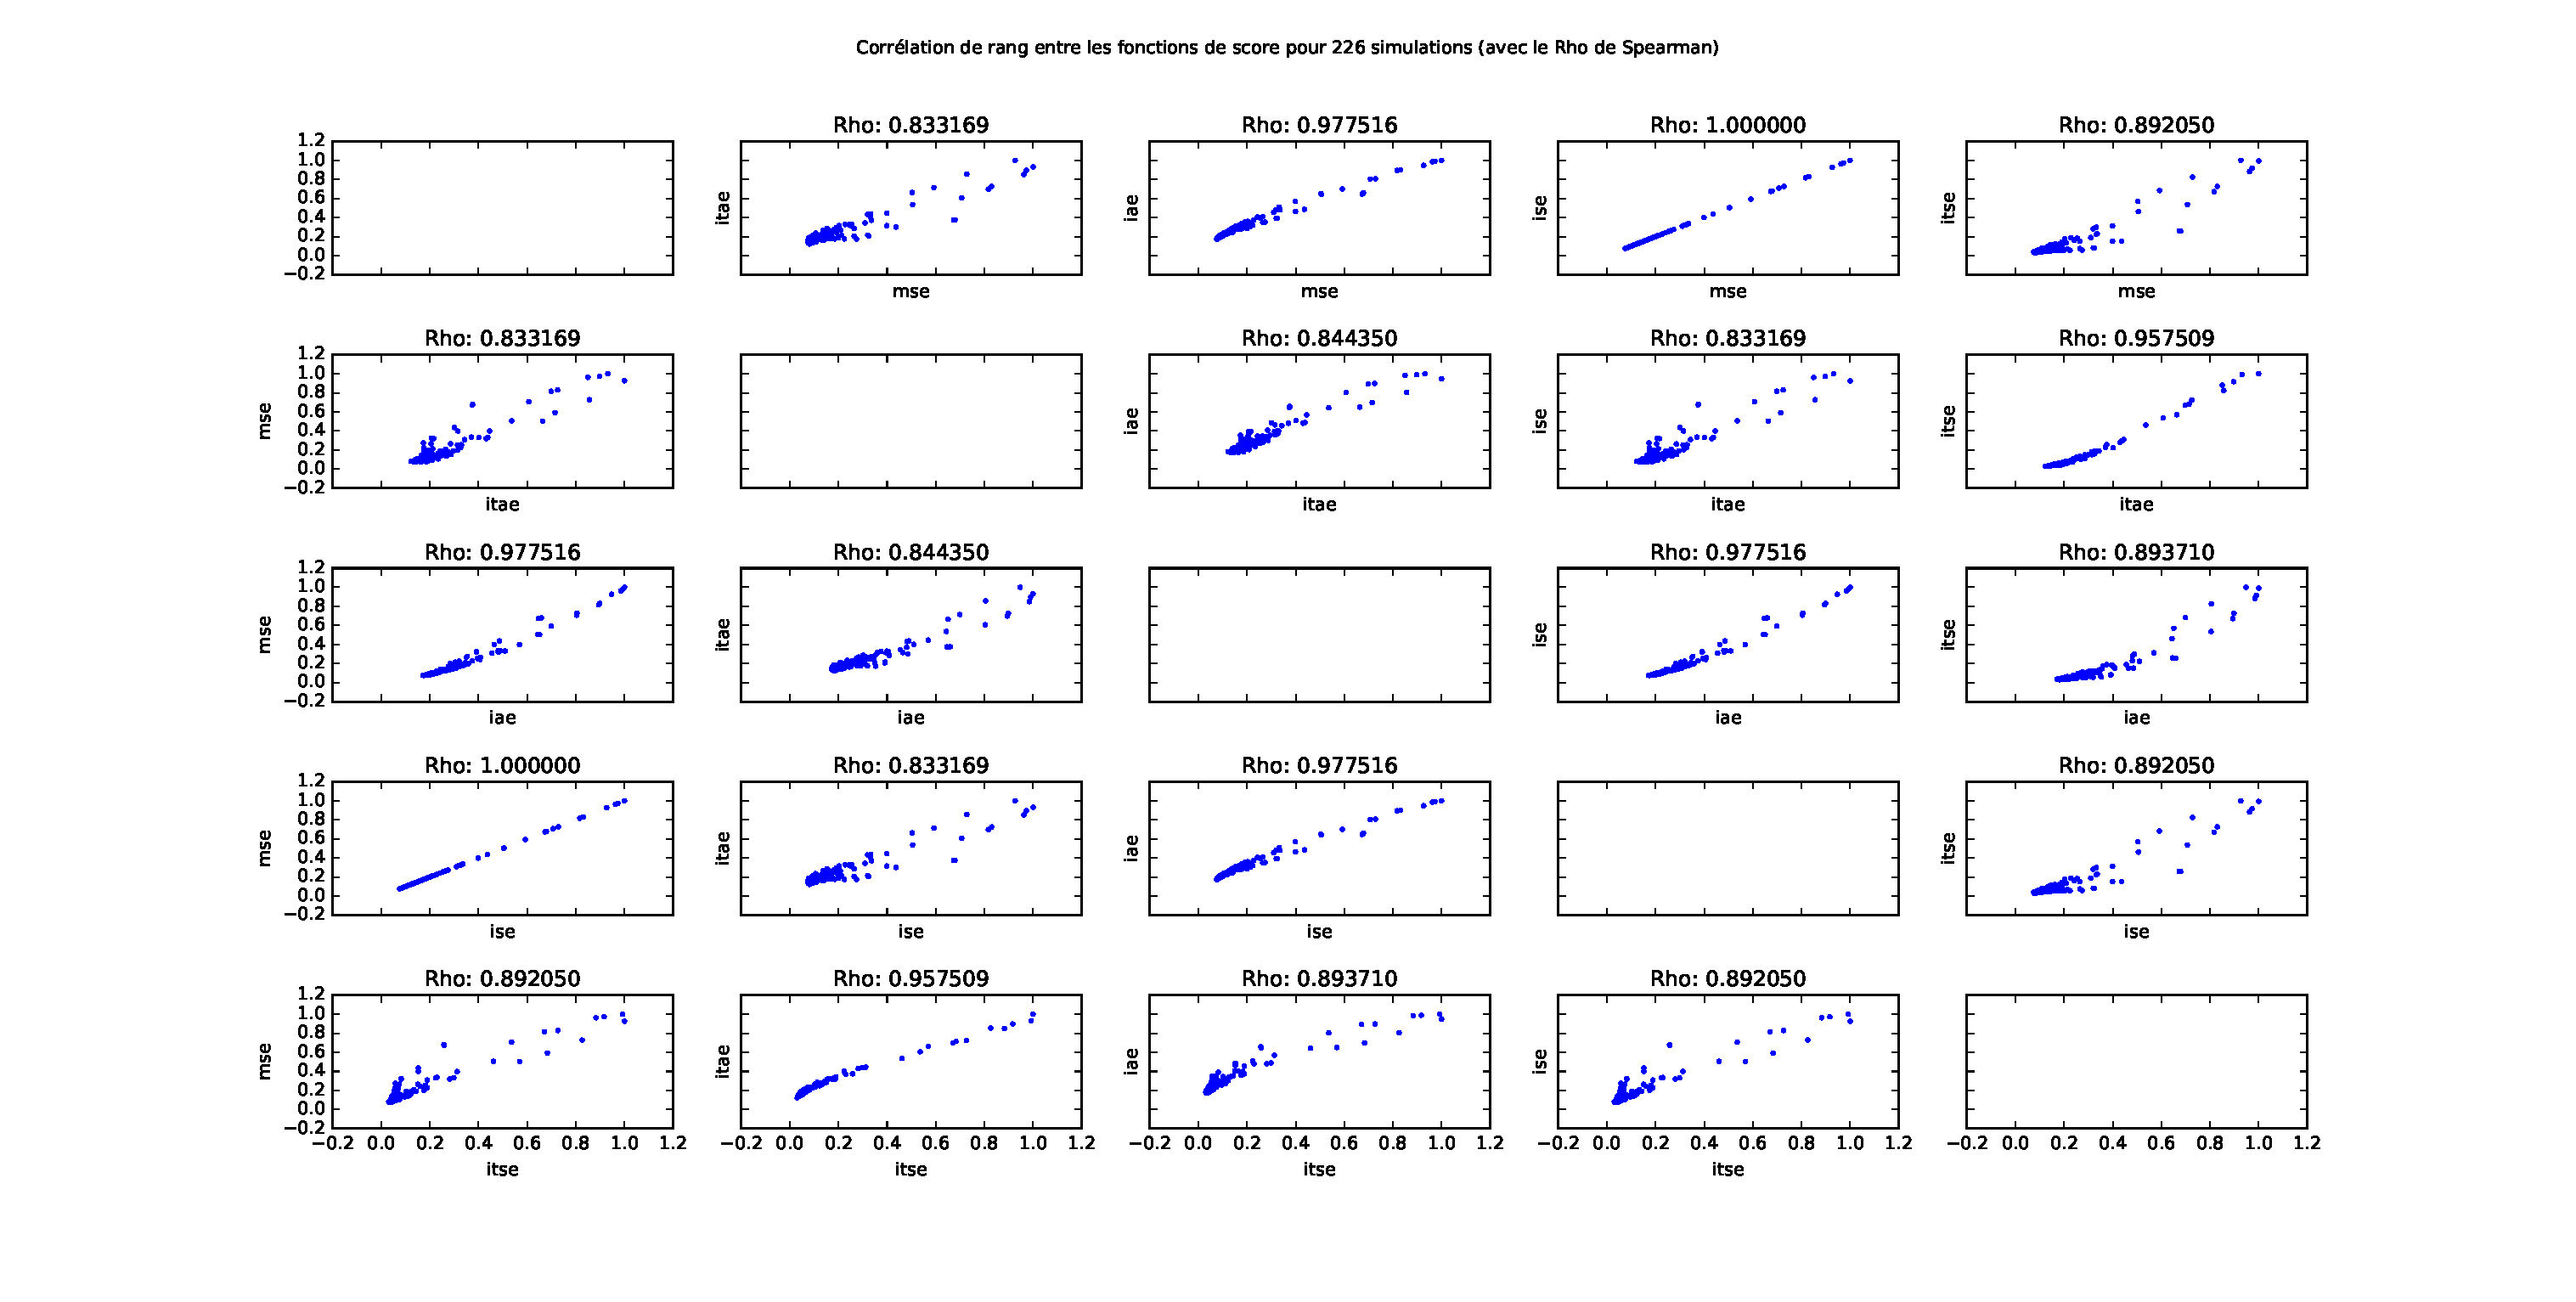
\includegraphics[scale=0.35]{correlation.eps}
   \caption{\label{fig:correlation} Corrélation de rang entre les différentes fonctions de score}
\end{figure}


\subsection{Méthodes de contrôle}

Nous avons ensuite comparé les différentes méthodes de contrôle décrites dans la section \ref{sec:contr-implem} ainsi que les variantes \textit{P} et \textit{PI} avec le protocole expérimental décrit dans la section \ref{sec:methode}.
PID et ses variantes ont été paramétrés grâce à la méthode de Ziegler-Nichols.

Nous avons obtenu les résultats suivants :

\begin{table}[H]
\begin{center}
    \begin{tabular}{|l|l|}
        \hline
        Bang Bang & $53,7 \cdot 10^4$ \\ \hline
        P         & $2,19 \cdot 10^4$ \\ \hline
        PI        & $2,23 \cdot 10^4$ \\ \hline
        PID       & $2,09 \cdot 10^4$ \\
        \hline
    \end{tabular}
\end{center}
\caption{Score des différents algorithmes de contrôle (moyenne sur 5 simulations)}
\end{table}


Comme nous pouvons le voir sur la figure en annexe \ref{fig:bangbang}, Bang-Bang ne fait qu'osciller au-dessus et en-dessous de la courbe, montrant clairement sa faiblesse pour contrôler des phénomènes non rémanents tels que l'intensité de la lumière.

L'algorithme P nous montre déjà sur la figure \ref{fig:p} un très bon contrôle de la lumière, oscillant faiblement aux alentours de la consigne.
Si la variable contrôlée ne nécessite pas une grande précision de contrôle, cette méthode peut-être largement suffisante et beaucoup plus facile à paramétrer, ne possédant qu'une seule constante à déterminer.

PI quant à lui, montre un contrôle moins bon que celui réalisé par l'algorithme P :
la courbe semble croître trop haut et prendre plus de temps pour s'aligner sur la valeur souhaitée.
Il est cependant à noter que la montée initiale est plus rapide que celle de P (voir la figure \ref{fig:pi}).

L'algorithme PID nous montre sur la figure \ref{fig:pid} un contrôle beaucoup plus précis, atteignant plus rapidement la consigne et plus stable.

\subsection{Détermination des paramètres}
L'algorithme PID ayant montré sa supériorité, il est important de pouvoir déterminer correctement ses trois paramètres.
Pour cela, nous avons comparé plusieurs méthodes et nous sommes parvenus aux résultats suivants :

\begin{table}[H]
\begin{center}
    \begin{tabular}{|l|l|}
        \hline
        Manuelle & $2,84 \cdot 10^4$ \\ \hline
        Ziegler-Nichols & $3,91 \cdot 10^4$ \\ \hline
        Génétique        & $2,22 \cdot 10^4$ \\ \hline
    \end{tabular}
\end{center}
\caption{Score de différentes méthodes de tuning de PID (moyenne sur 5 simulations)}

\end{table}

\subsubsection{Méthode manuelle}

La méthode manuelle, illustrée sur la figure en annexe \ref{fig:manuelle}, montre une courbe croissant assez lentement vers la consigne, mais restant relativement stable à ses alentours. Même si ces résultats sont assez bons, cette méthode présente le désavantage de nécessiter la présence d'un technicien, ce qui peut prendre un temps considérable si les réactions du phénomène sont lentes.

\subsubsection{Méthode de Ziegler-Nichols}

La méthode de Ziegler-Nichols, illustrée sur la figure \ref{fig:ziegler}, montre elle-aussi d'assez bons résultats, mais reste cependant la moins bonne des trois méthodes utilisées.
Sa croissance initiale est moins rapide et ses variations un peu plus grandes, mais elle fut bien plus simple et rapide à appliquer, car une fois la courbe attendue obtenue, il suffit d'appliquer trois opérations pour connaître les valeurs des paramètres.

\subsubsection{Algorithme génétique}
L'utilisation d'un algorithme génétique, illustrée sur la figure en annexe \ref{fig:genetique}, montre également une croissance très rapide vers la consigne et des oscillations qui restent très proches de celle-ci.
Son score est également le plus bas, indiquant le meilleur contrôle.

Il s'agit cependant la méthode qui aura pris le plus de temps pour déterminer les paramètres, mais à l'avantage de ne nécessiter aucun technicien et d'être facilement parallélisable.

Nous avons fait tourner notre algorithme génétique pendant 14 générations avec 50 chromosomes par génération.

Nous pouvons voir une convergence du score assez rapide dans notre cas pour la détermination des paramètres, comme indiqués sur la figure \ref{fig:convergence}.

De plus, quand nous observons uns à uns les paramètres des chromosomes au cours des générations, nous observons que ceux-ci convergent individuellement vers une valeur optimale comme nous pouvons le voir dans la figure \ref{fig:kibox}.


\chapter{Conclusion et perspectives}

Nous pouvons constater qu'en fonction du phénomène à contrôler, les différents algorithmes analysés présentent des avantages et inconvénients.
En effet, pour des phénomènes rémanents tels que la diffusion de chaleur, Bang bang est amplement suffisant.
Par contre, pour des phénomènes spontanés comme la luminosité, nécessitent un contrôle plus subtile jouant sur l'intensité, et c'est là que PID montre tout son intérêt.

Nos résultats montrent que malgré la facilité de paramétrisation de P et PI, PID reste le  plus efficace dans le contrôle.

Cependant, celui-ci doit être bien calibré.
Nous avons donc comparé plusieurs techniques de calibrations.
Nous avons démontré que parmi ces techniques de calibrations, les trois présentent des avantages et inconvénients:
\begin{itemize}
    \item La méthode manuelle peut donner un résultat assez précis mais nécessite l'action d'un technicien lors de la calibration
    \item Ziegler-Nichols est plus rapide a exécuter mais donne des résultats moins précis.
    \item L'algorithme génétique donne les meilleurs résultats mais nécessite beaucoup de temps. Cependant, il ne requière guère aucune interaction humaine.
\end{itemize}

La mise en situation réelle lors du Printemps des Sciences nous a permis de tester nos algorithmes et résultats. La serre était suffisamment réactive lors des perturbations simulées pendant les démonstrations faites aux visiteurs, et la correction était faite de façon rapide et efficace.

Ce projet aurait pu être étendu de plusieurs manières:

\begin{enumerate}
\item Premièrement, il aurait été possible d'implémenter le contrôleur MPC, mais celui-ci demandait plus de ressources matérielles.
\item Pour ce qui est des méthodes de sélection des paramètres de PID, il serait possible d'automatiser entièrement l'algorithme de Ziegler-Nichols. En effet, actuellement celui-ci est automatique à l'exception d'une interaction humaine ponctuelle lors de la phase de détection d'oscillations. Une approche plus automatisée de celles-ci aurait pu être créée pour améliorer l'algorithme Ziegler-Nichols. Également, l'algorithme génétique aurait pu être amélioré en raffinant pour qu'il y ait des différences de probabilité, au niveau du taux de crossing-over et de mutation, entre générations.
\item Côté hardware, il aurait été possible d'améliorer les circuits pour réduire le phénomène de bruit. Ce bruit était parfois légèrement représentatif, donc un filtrage hardware et/ou software (tel qu'un filtre de Kalman) aurait pu être envisagé (PID fonctionnant mieux sans bruit).
\end{enumerate}


\bibliographystyle{apalike}

\bibliography{biblio}
\addcontentsline{toc}{chapter}{Bibliographie}

\appendix

\chapter{Graphes des simulations intéressantes}

\pagenumbering{gobble} % Stopper la numérotation de pages

Cette annexe sert de support aux conclusions auxquelles nous sommes arrivés dans le chapitre \ref{chap:res} et présente des graphes des simulations que nous avons considéré comme intéressantes.

\begin{figure}[htb!]
   \centering
   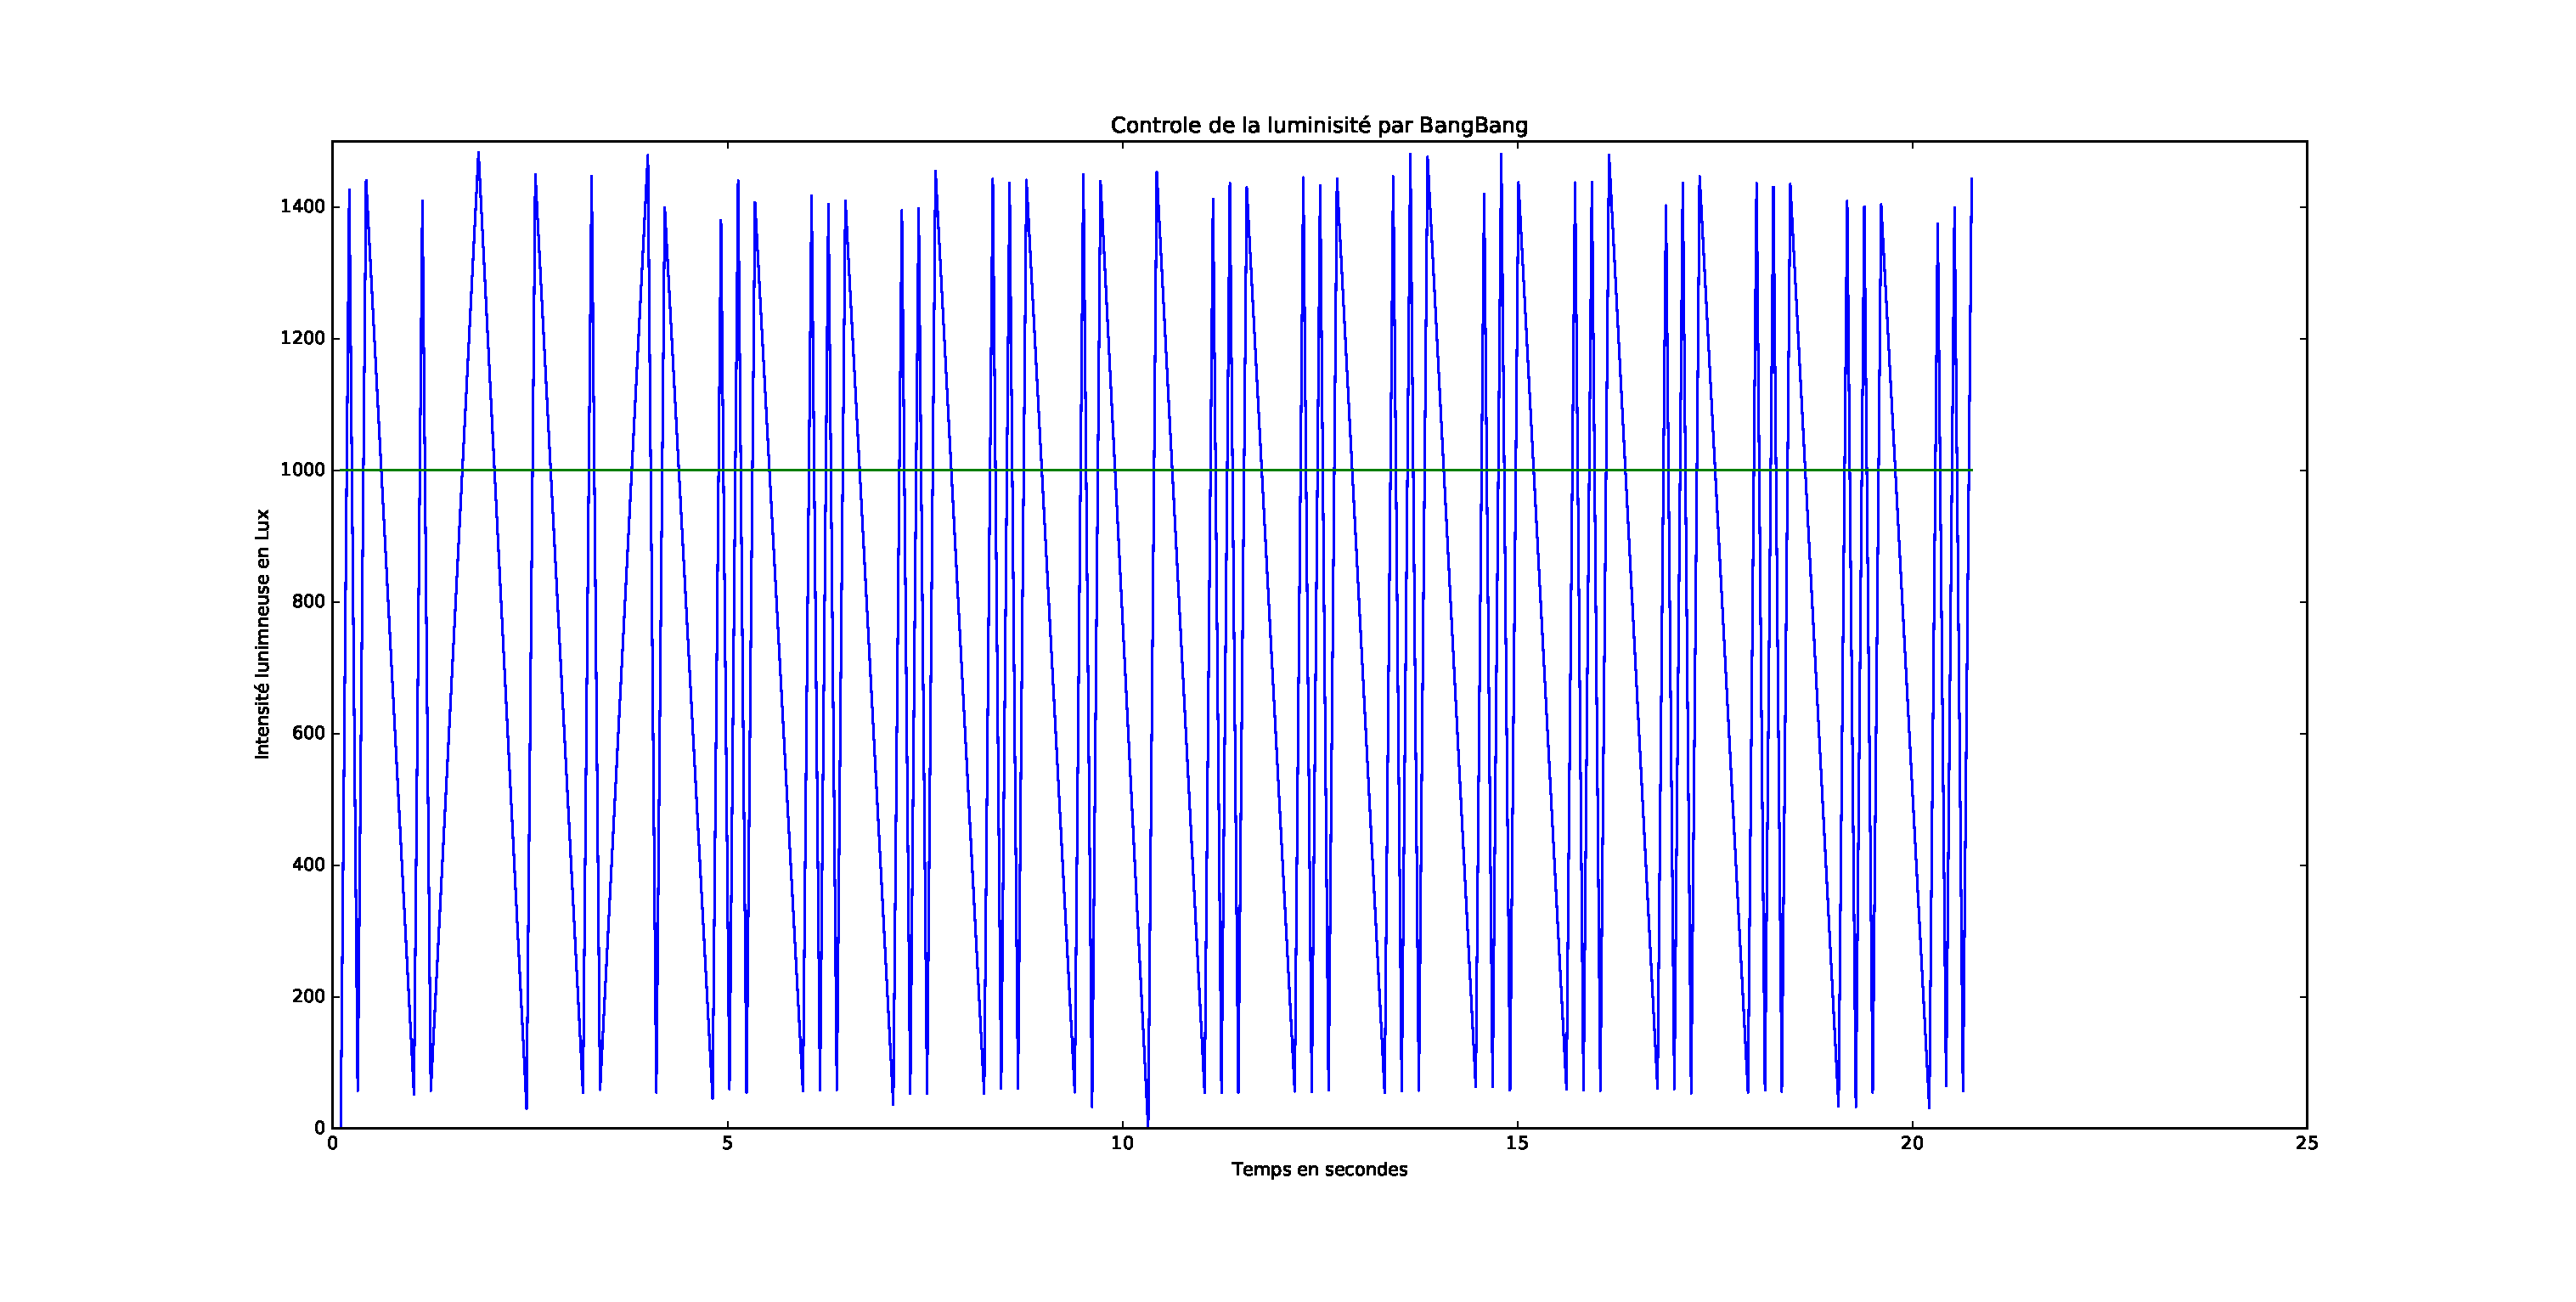
\includegraphics[scale=0.35]{BangBang.eps}
   \caption{\label{fig:bangbang} Contrôle de la luminosité par BangBang}
\end{figure}

\begin{figure}[htb!]
   \centering
   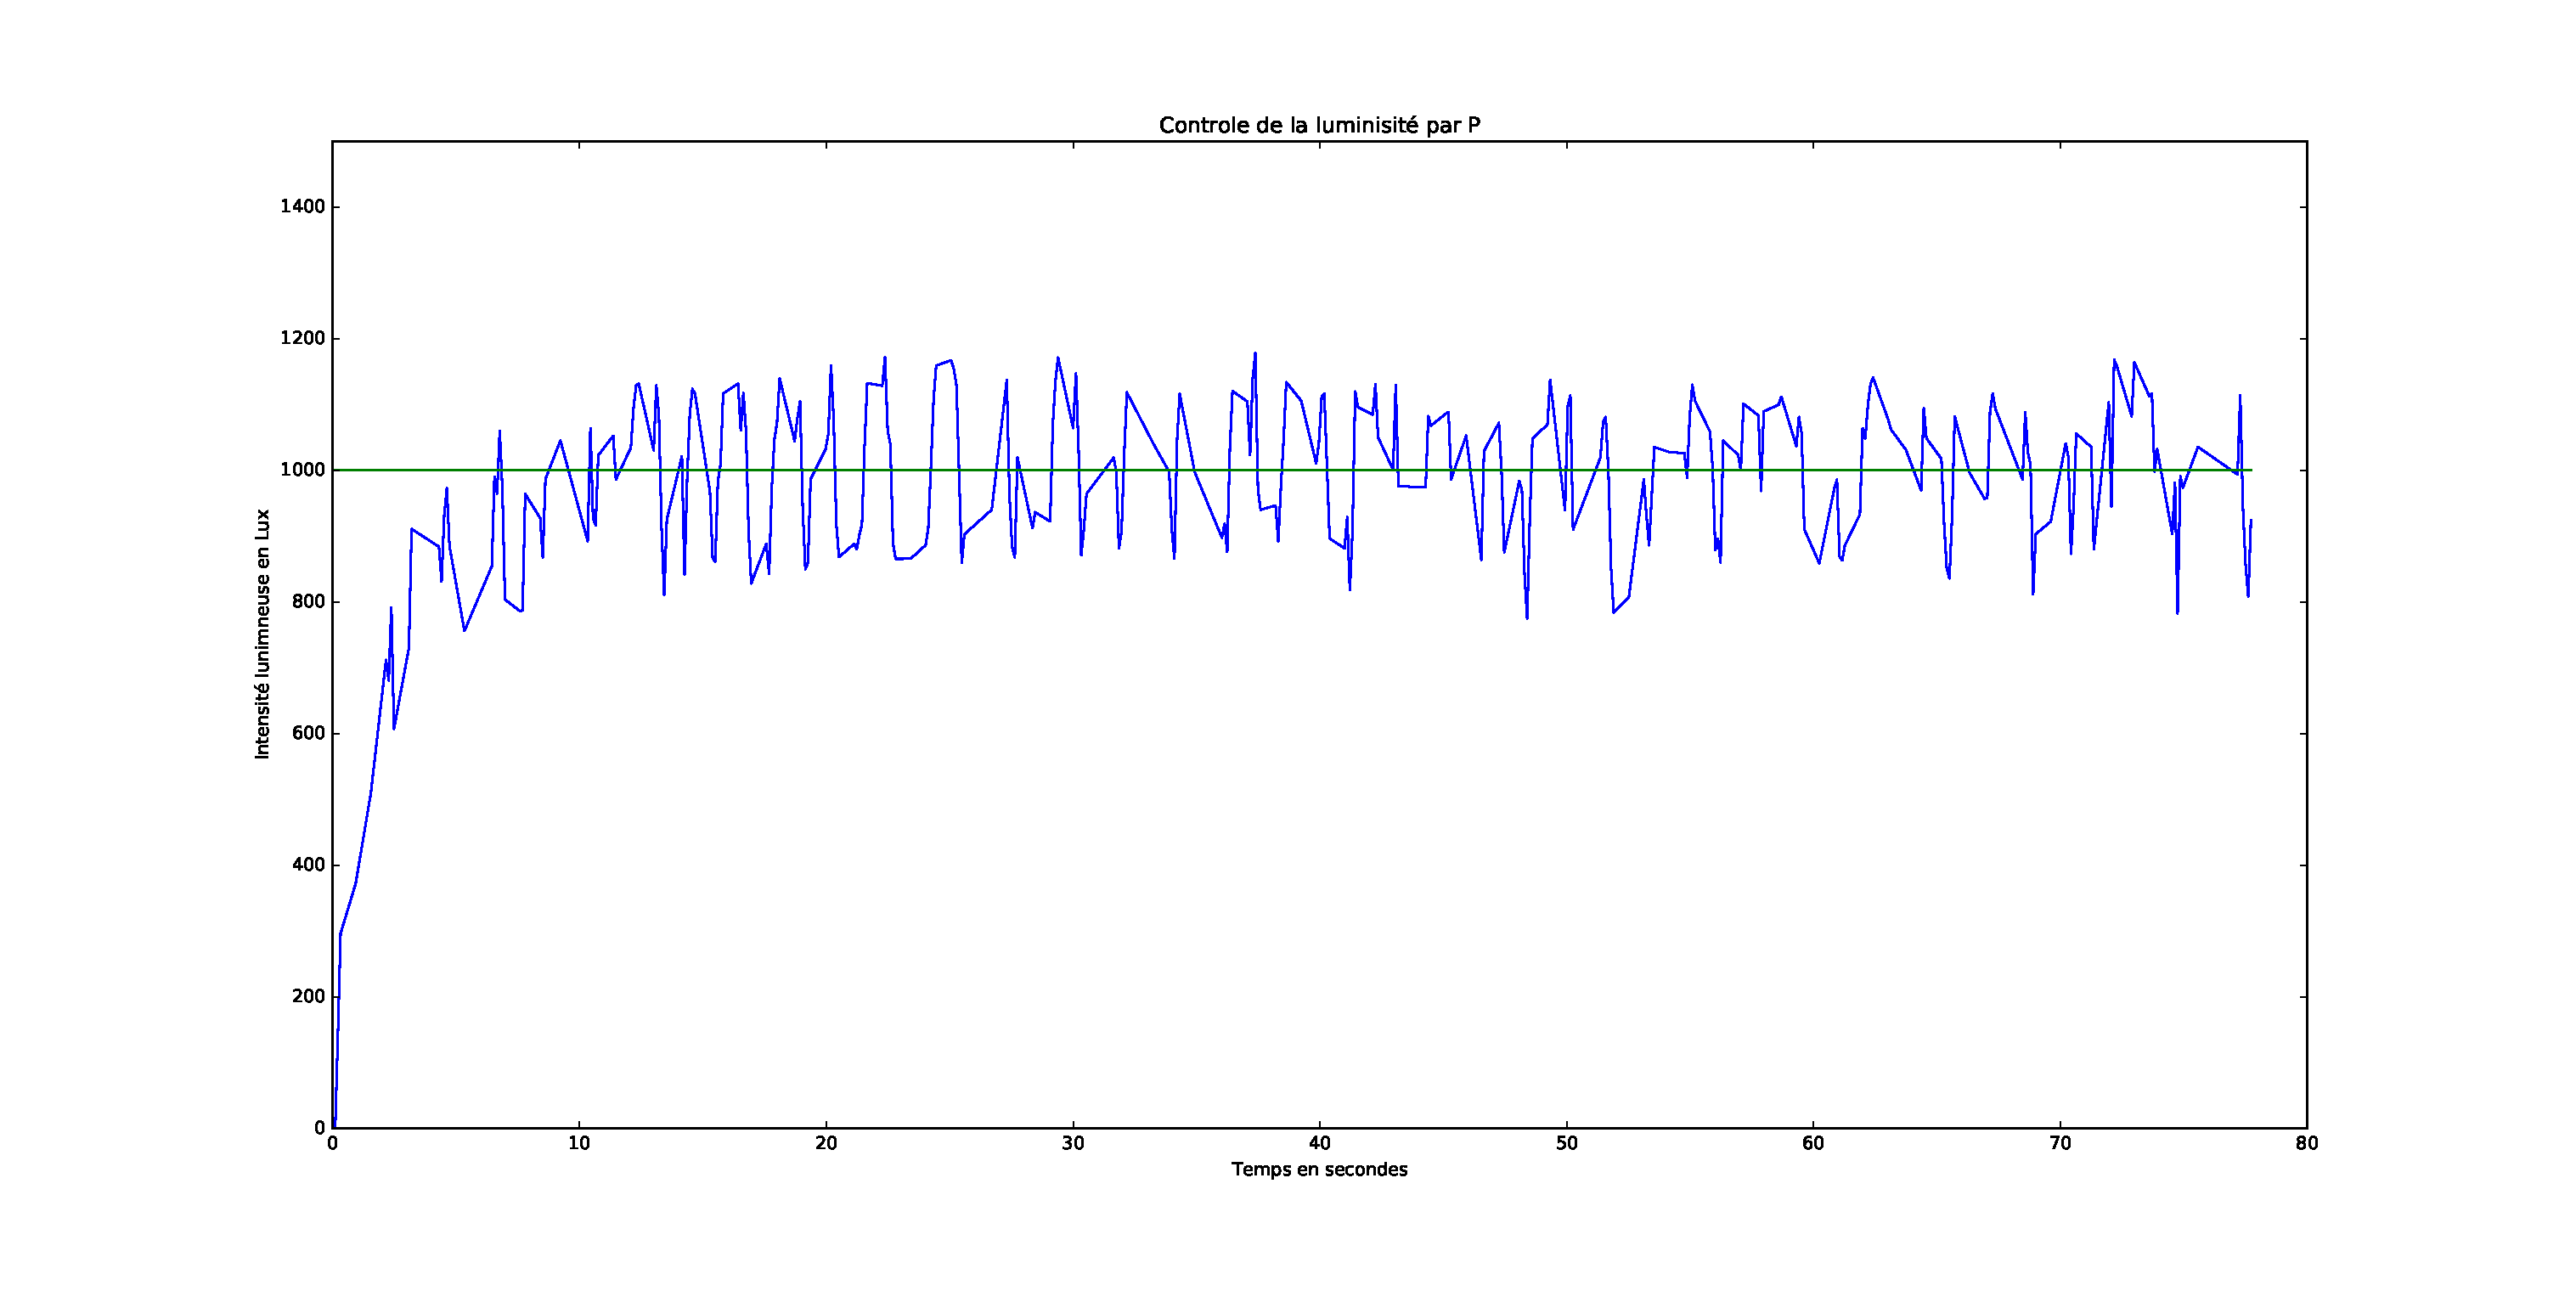
\includegraphics[scale=0.35]{P.eps}
   \caption{\label{fig:p} Contrôle de la luminosité par P}
\end{figure}

\begin{figure}[htb!]
   \centering
   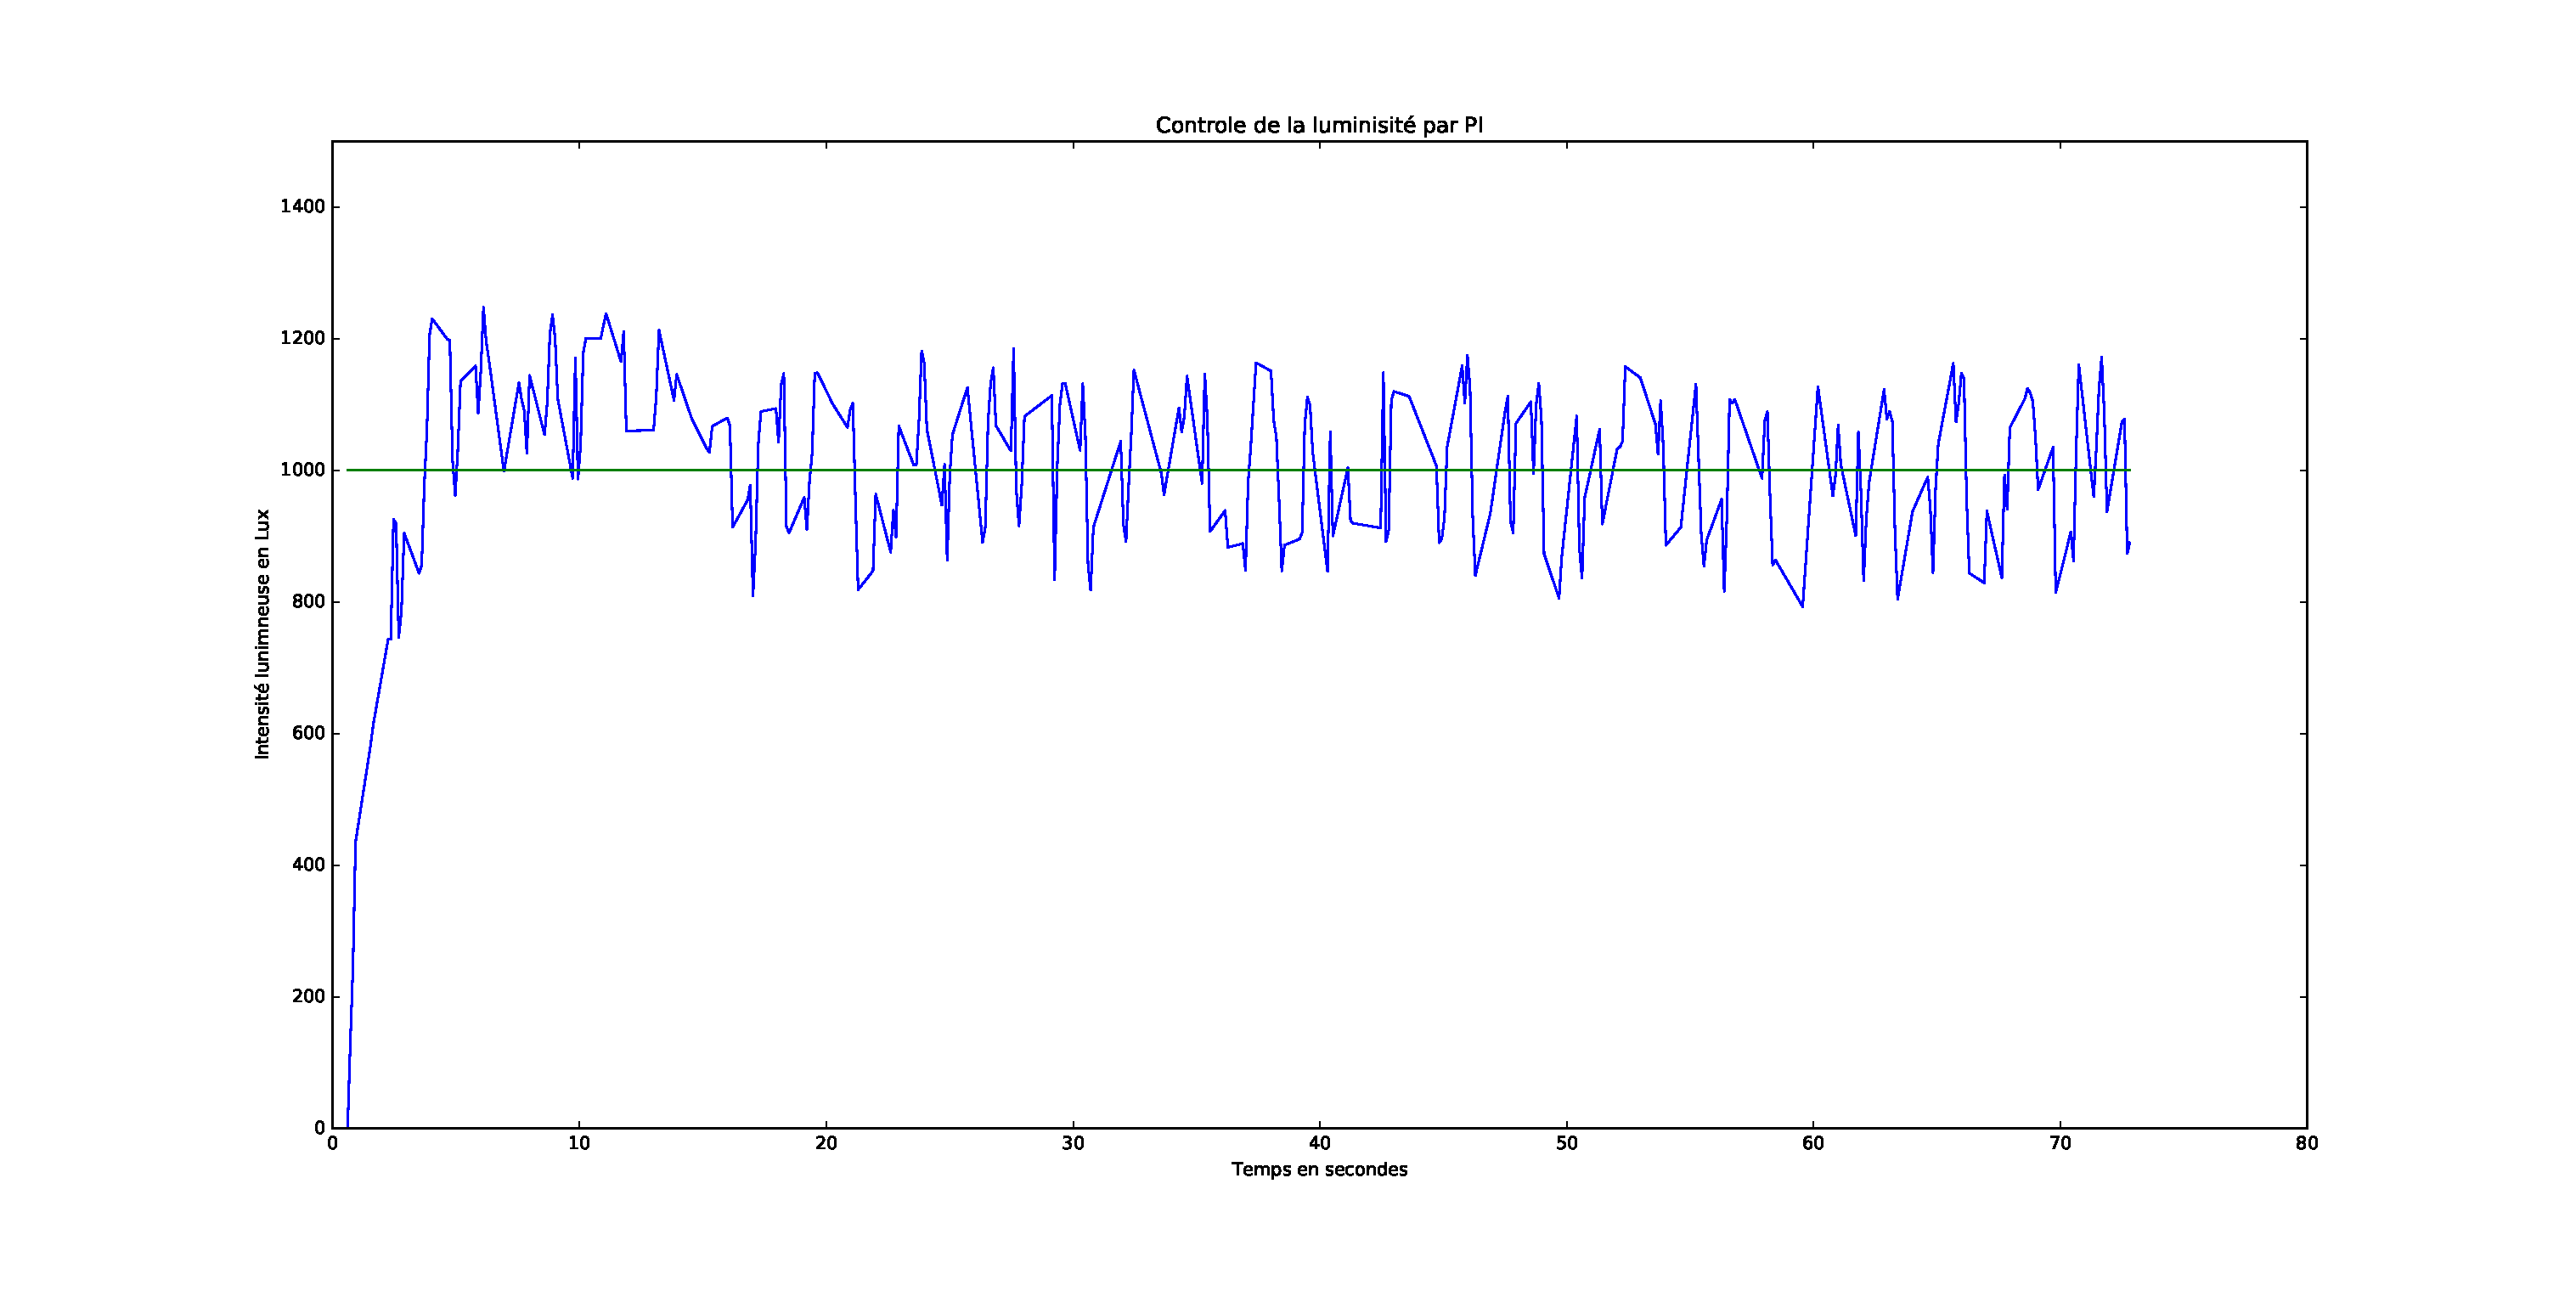
\includegraphics[scale=0.35]{PI.eps}
   \caption{\label{fig:pi} Contrôle de la luminosité par PI}
\end{figure}

\begin{figure}[htb!]
   \centering
   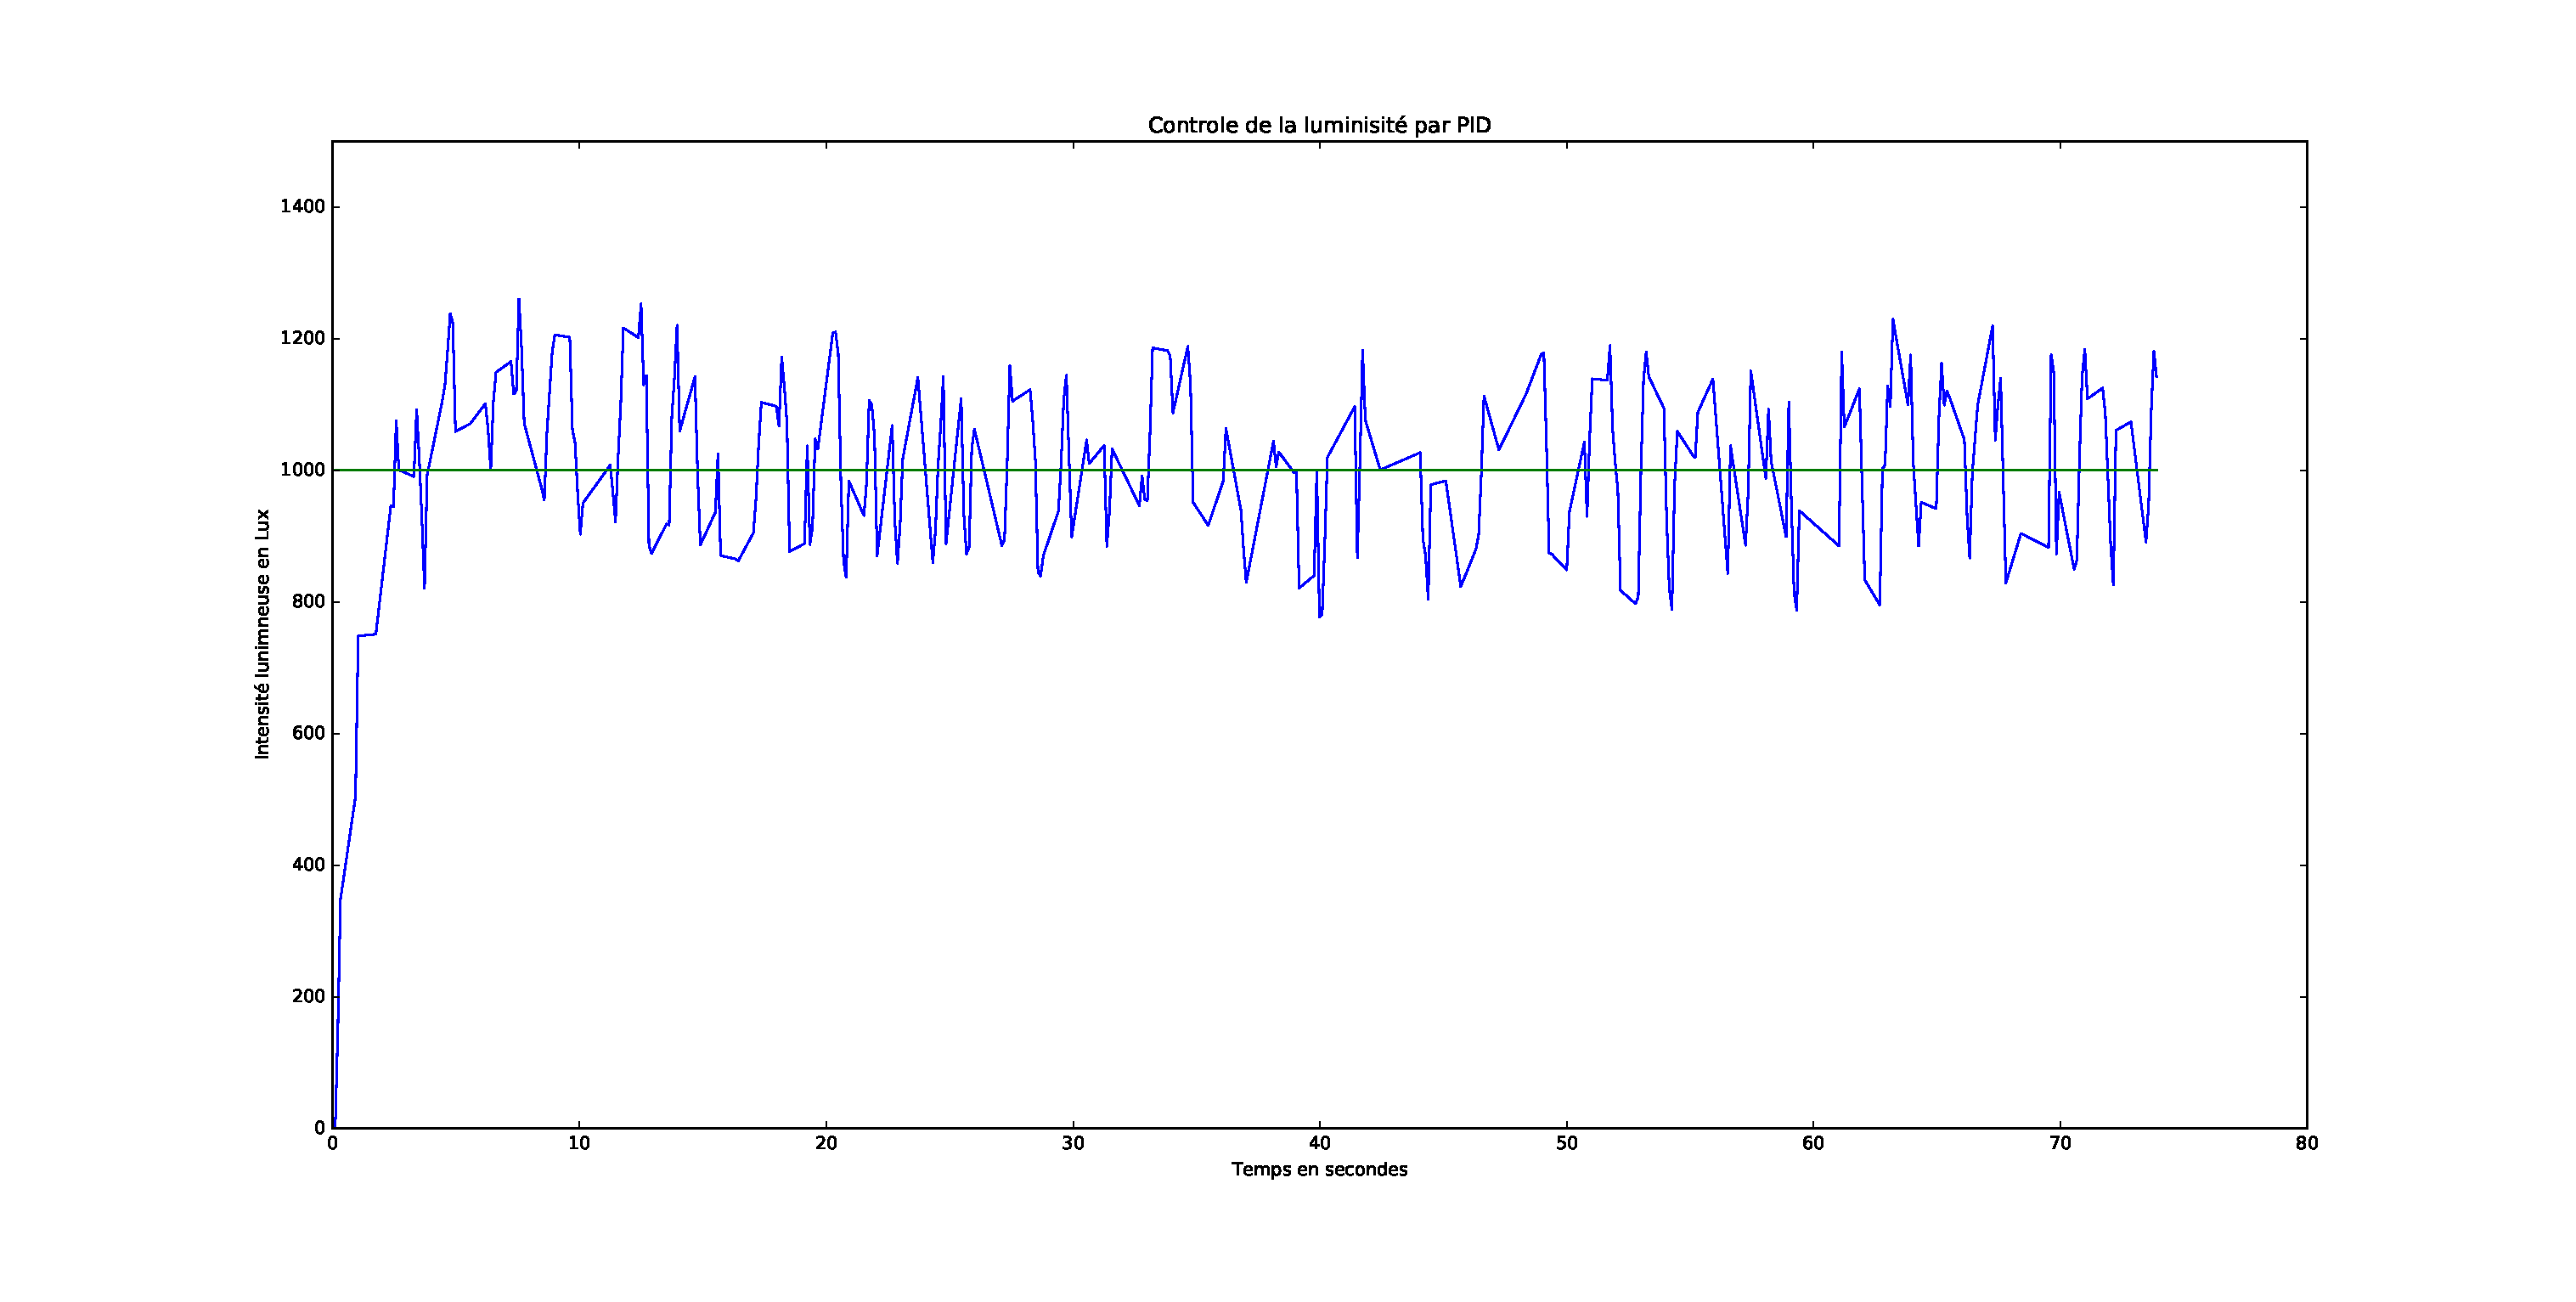
\includegraphics[scale=0.35]{PID.eps}
   \caption{\label{fig:pid} Contrôle de la luminosité par PID}
\end{figure}

\begin{figure}[htb!]
   \centering
   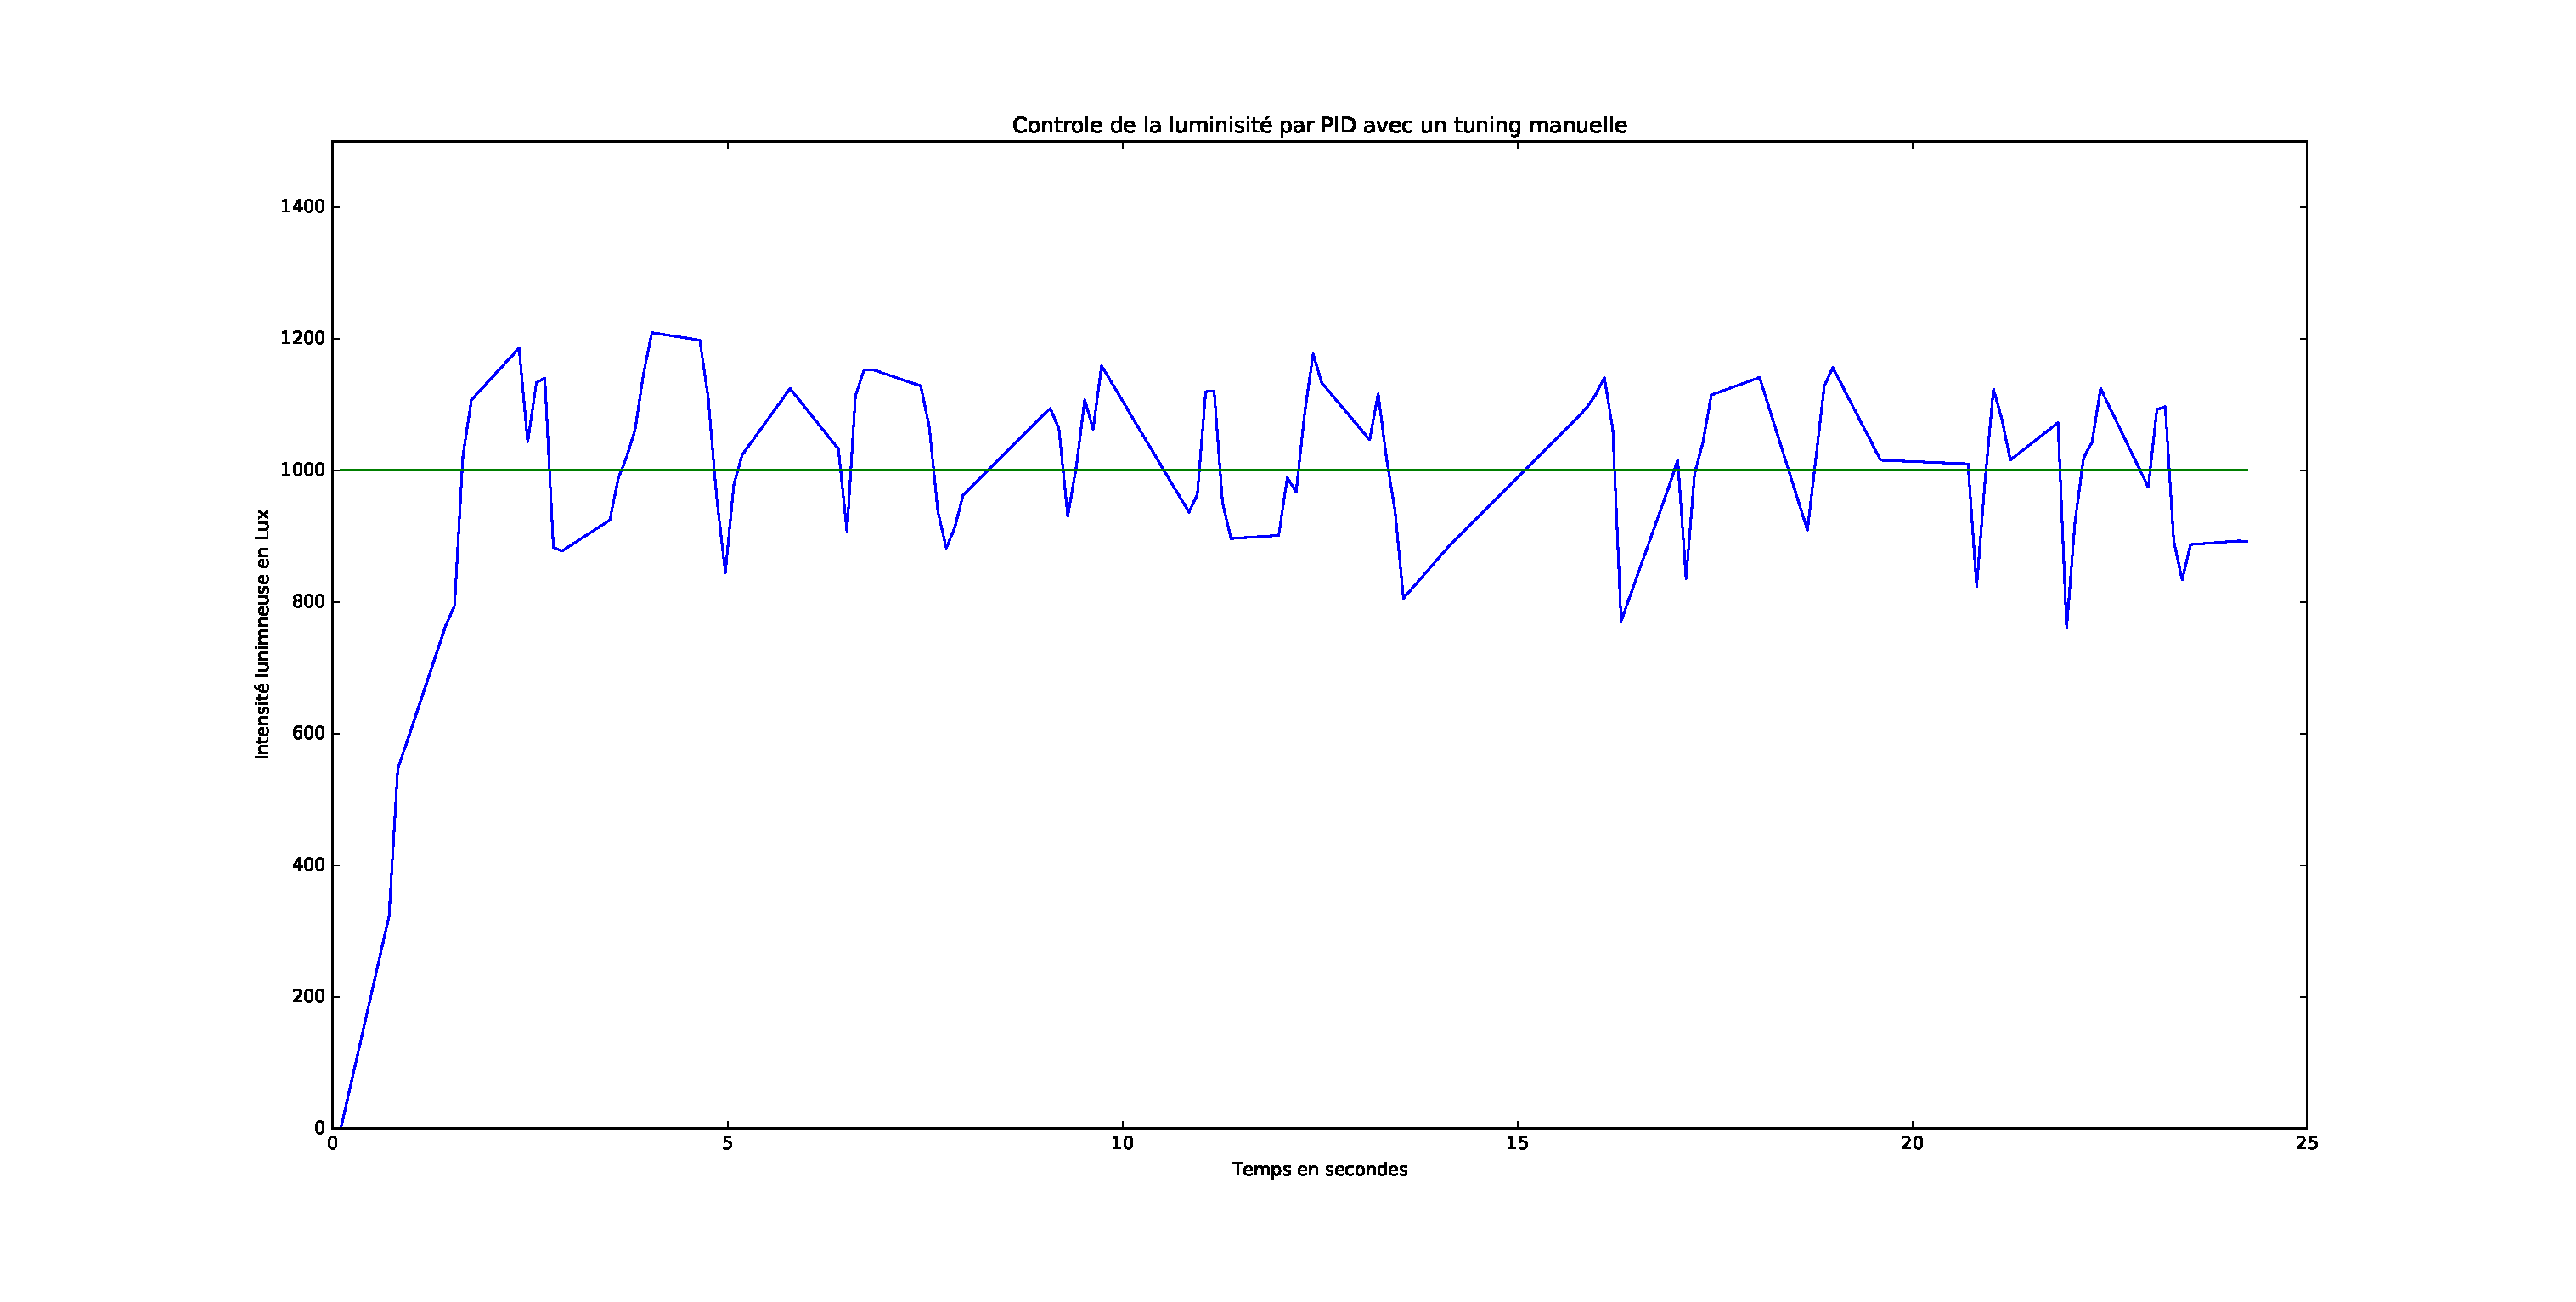
\includegraphics[scale=0.35]{Manuelle.eps}
   \caption{\label{fig:manuelle} Contrôle de la luminosité avec PID paramétré à la main}
\end{figure}

\begin{figure}[htb!]
   \centering
   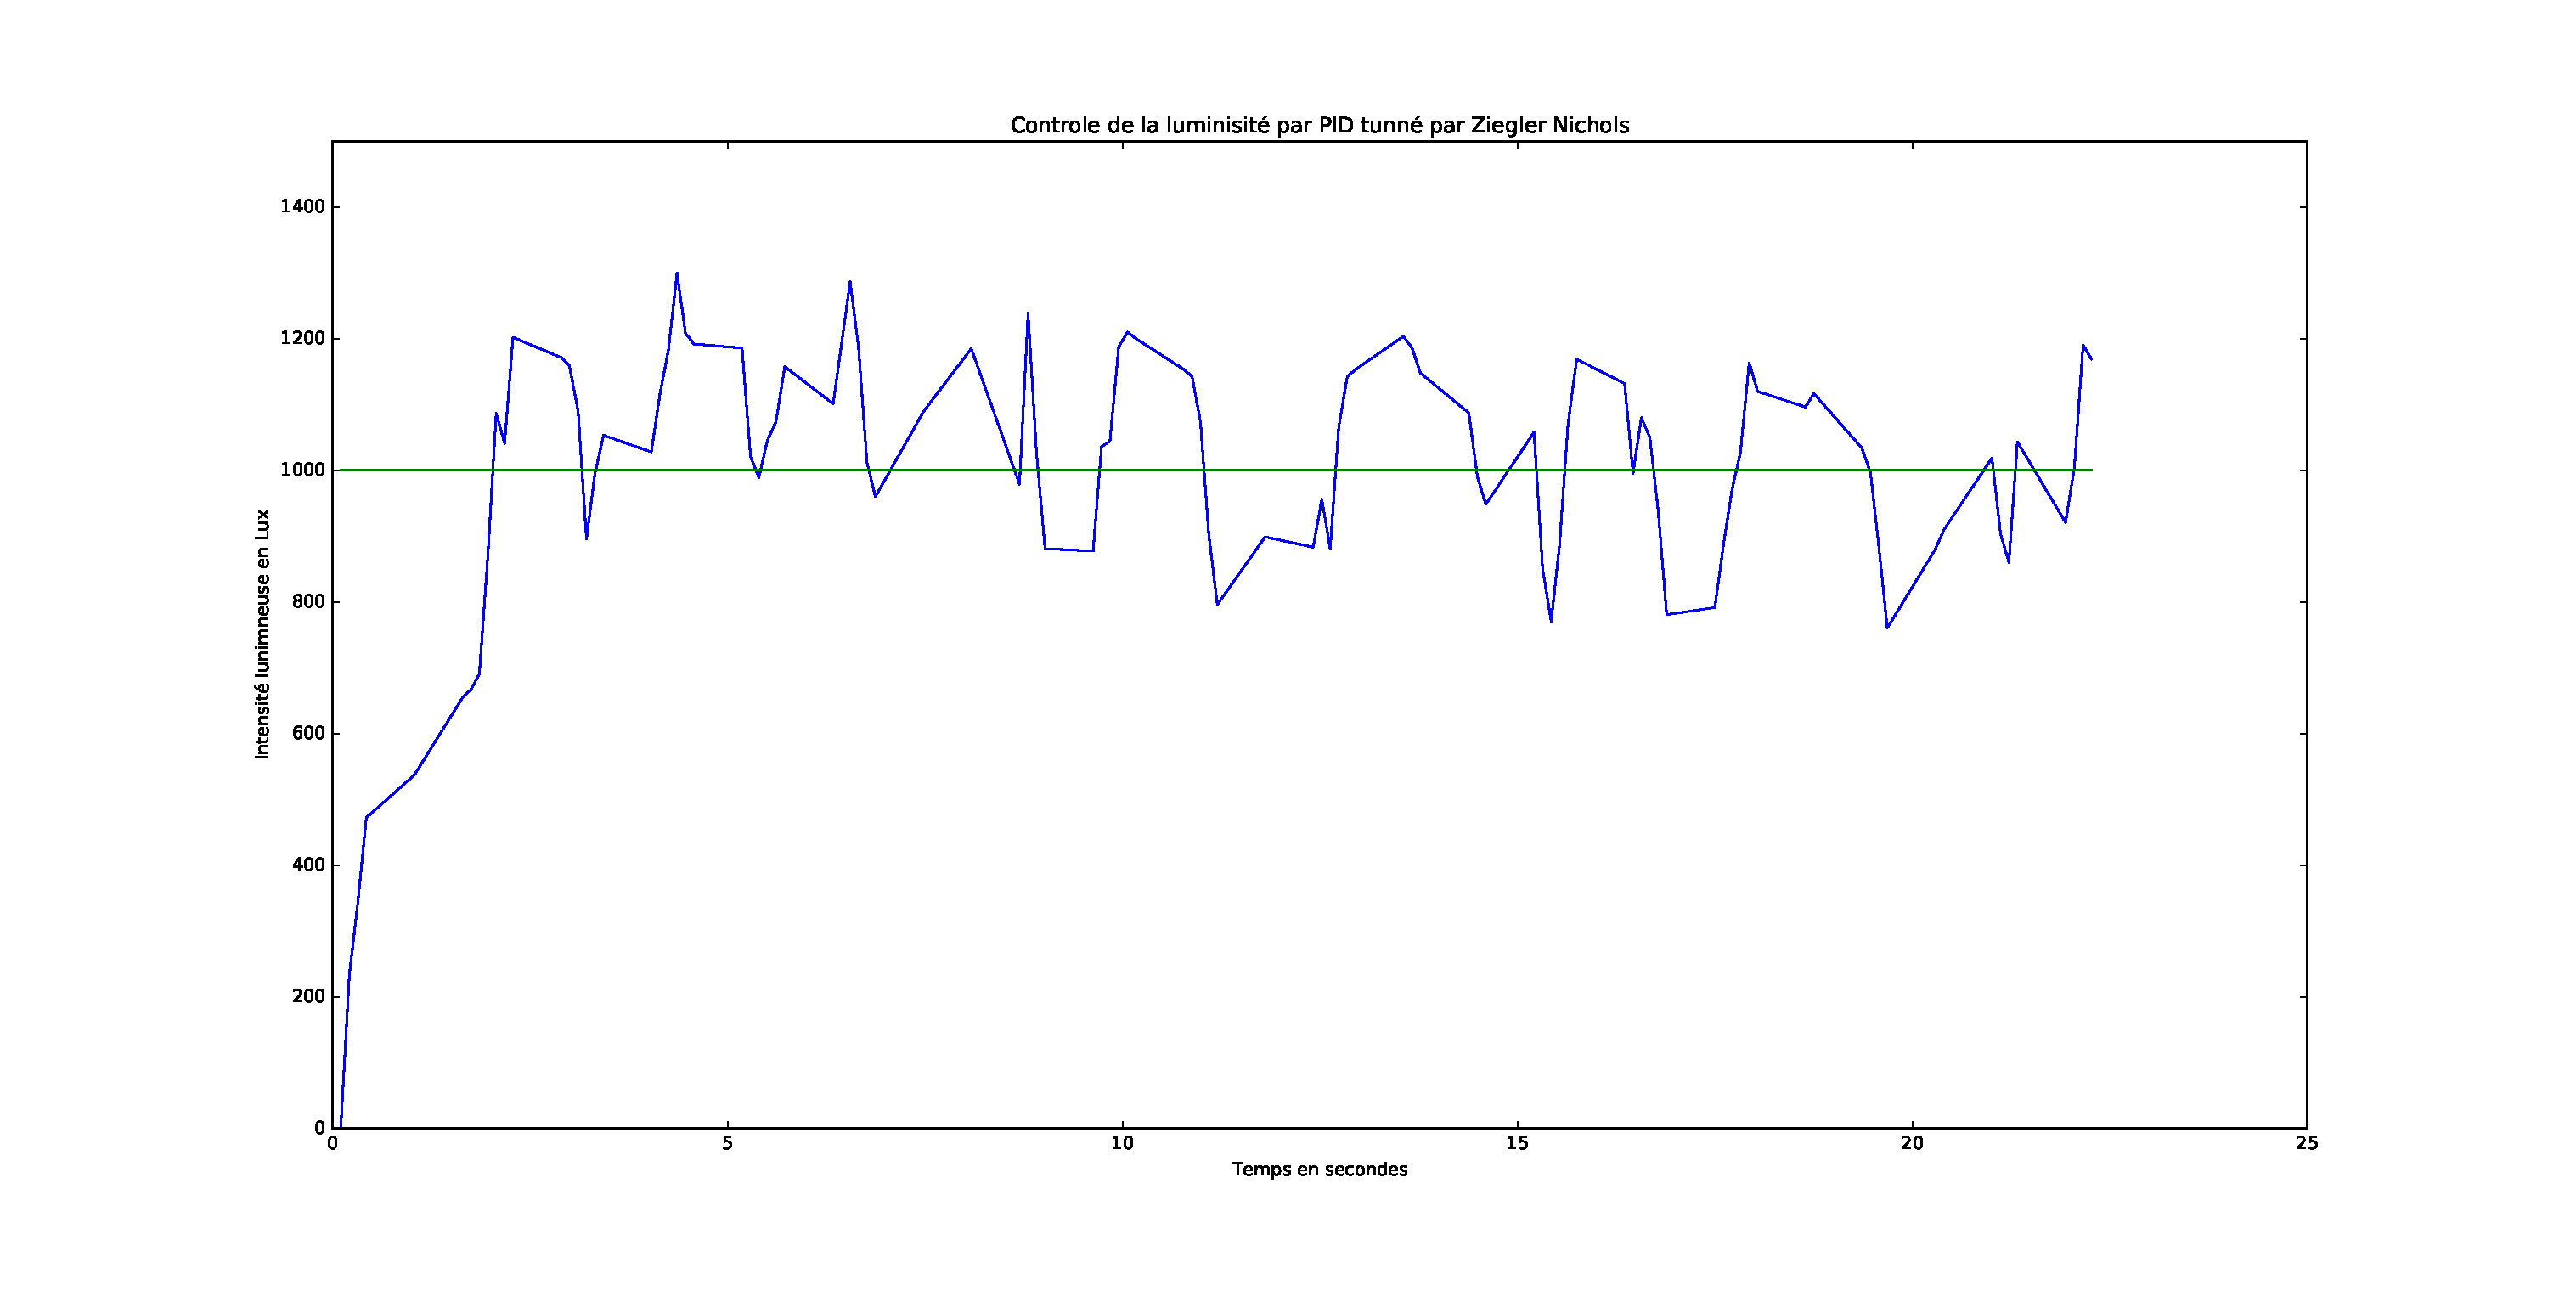
\includegraphics[scale=0.35]{Ziegler.eps}
   \caption{\label{fig:ziegler} Contrôle de la luminosité avec PID paramétré avec Ziegler-Nichols}
\end{figure}

\begin{figure}[htb!]
   \centering
   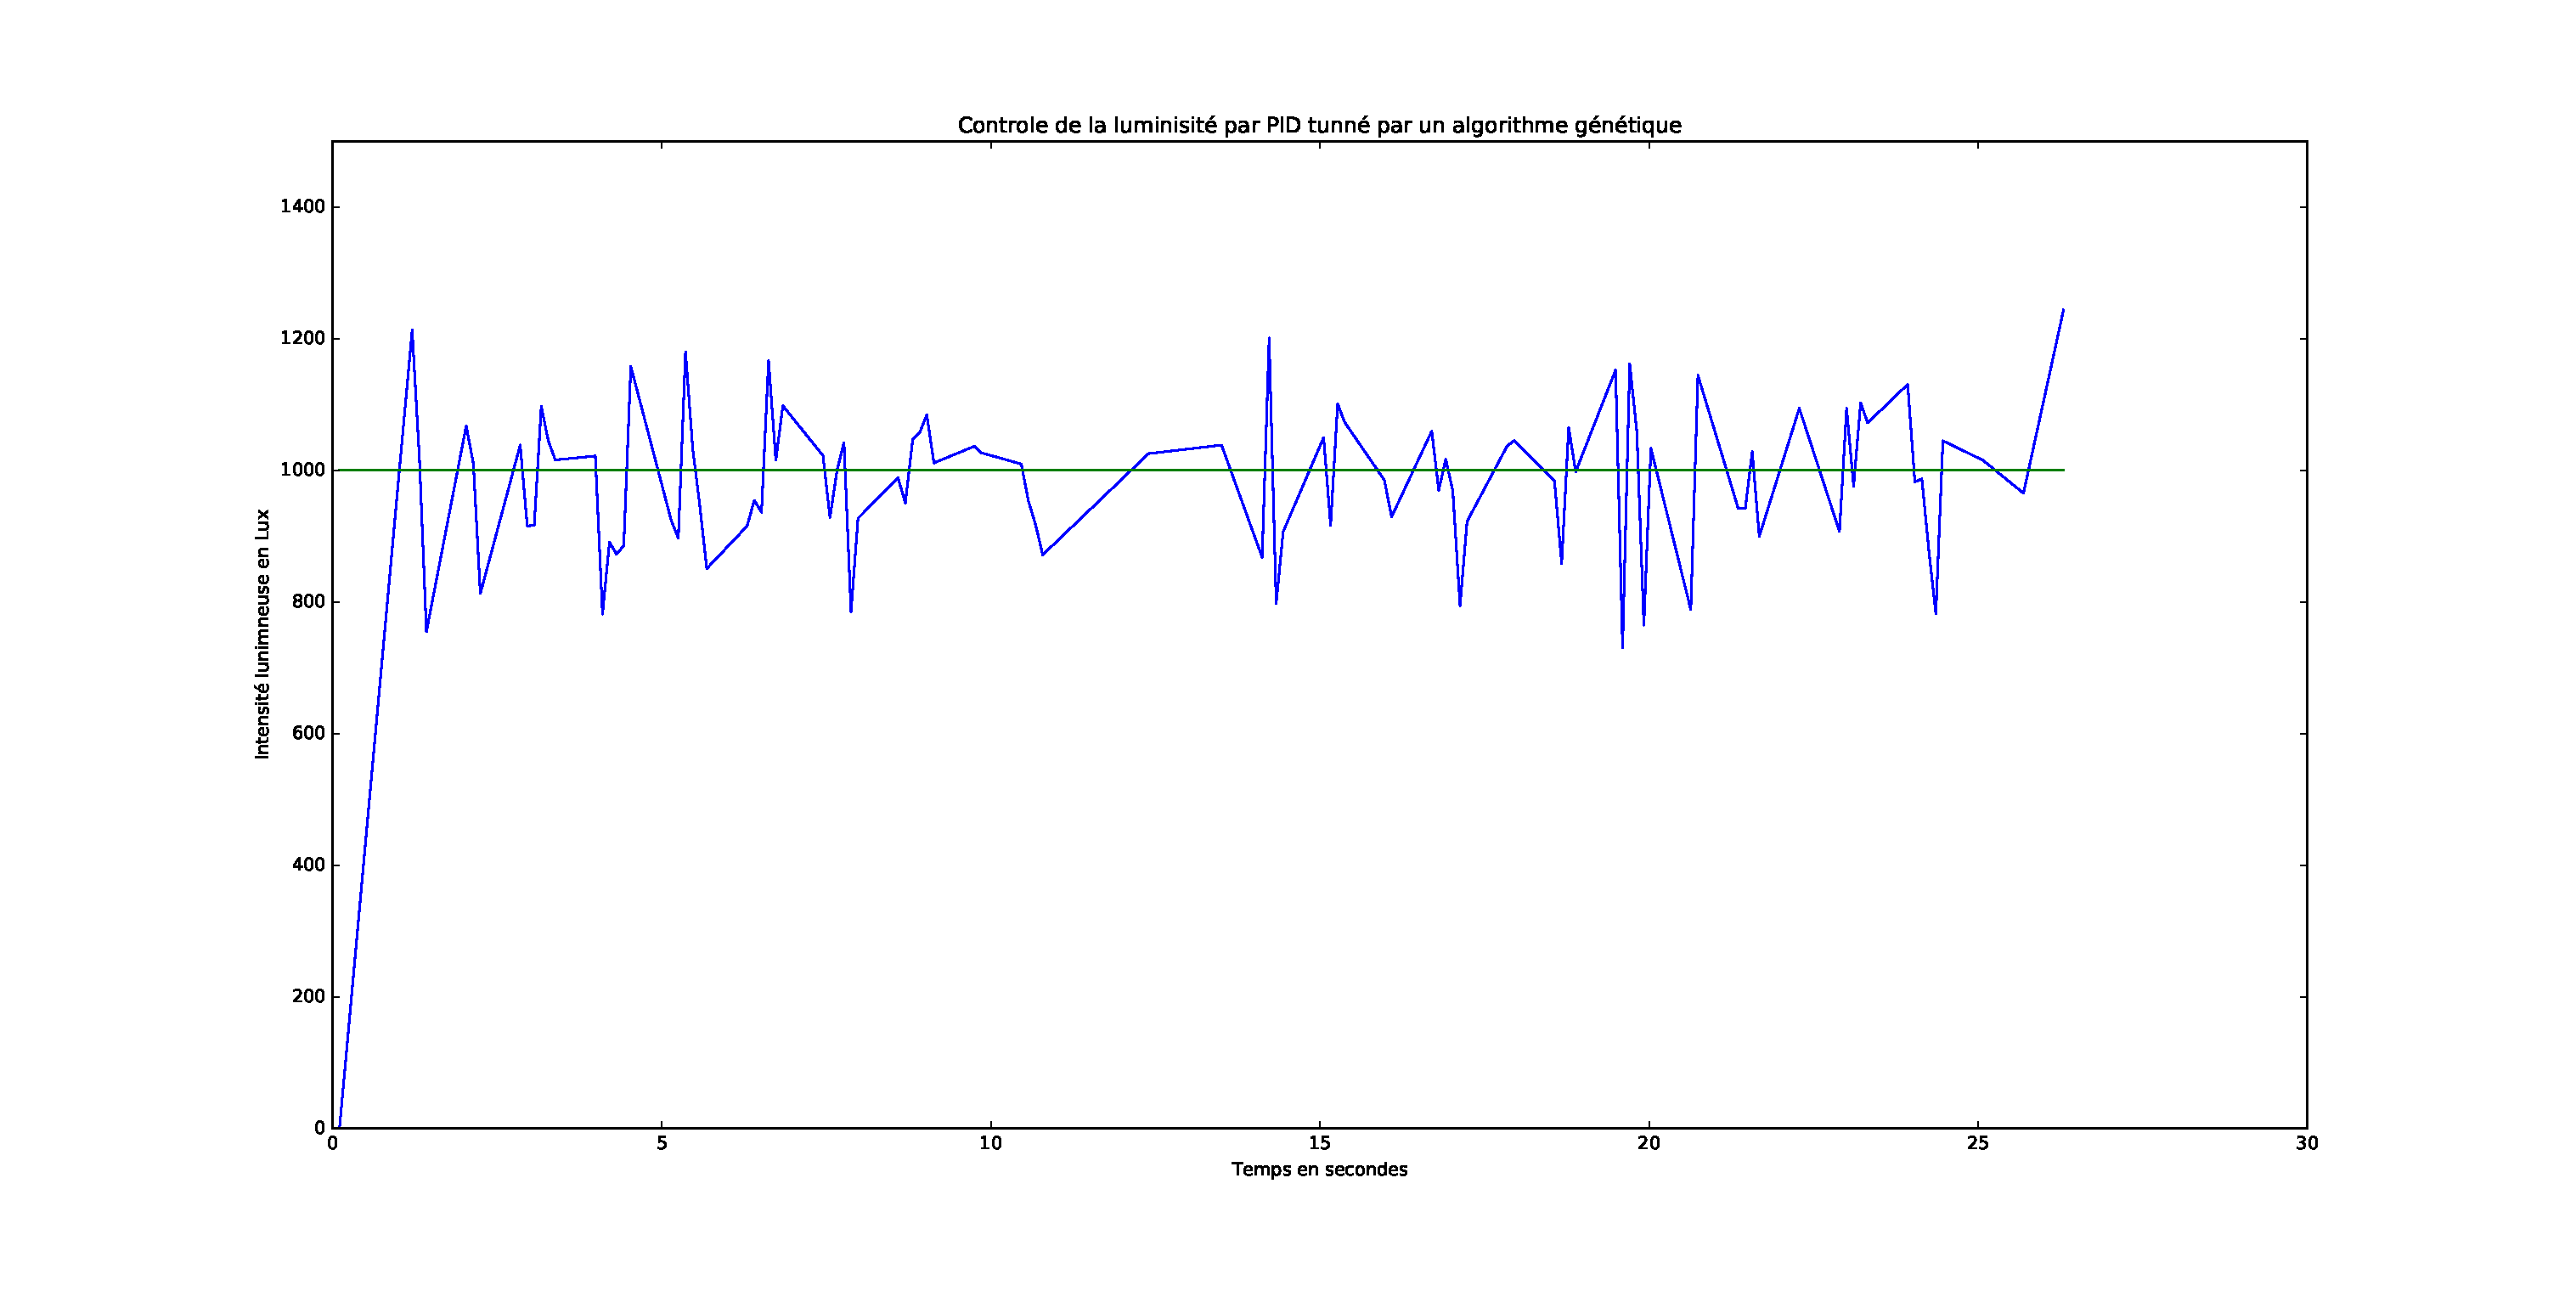
\includegraphics[scale=0.35]{Genetic.eps}
   \caption{\label{fig:genetique} Contrôle de la luminosité avec PID paramétré avec un algorithme génétique}
\end{figure}

\begin{figure}[htb!]
   \centering
   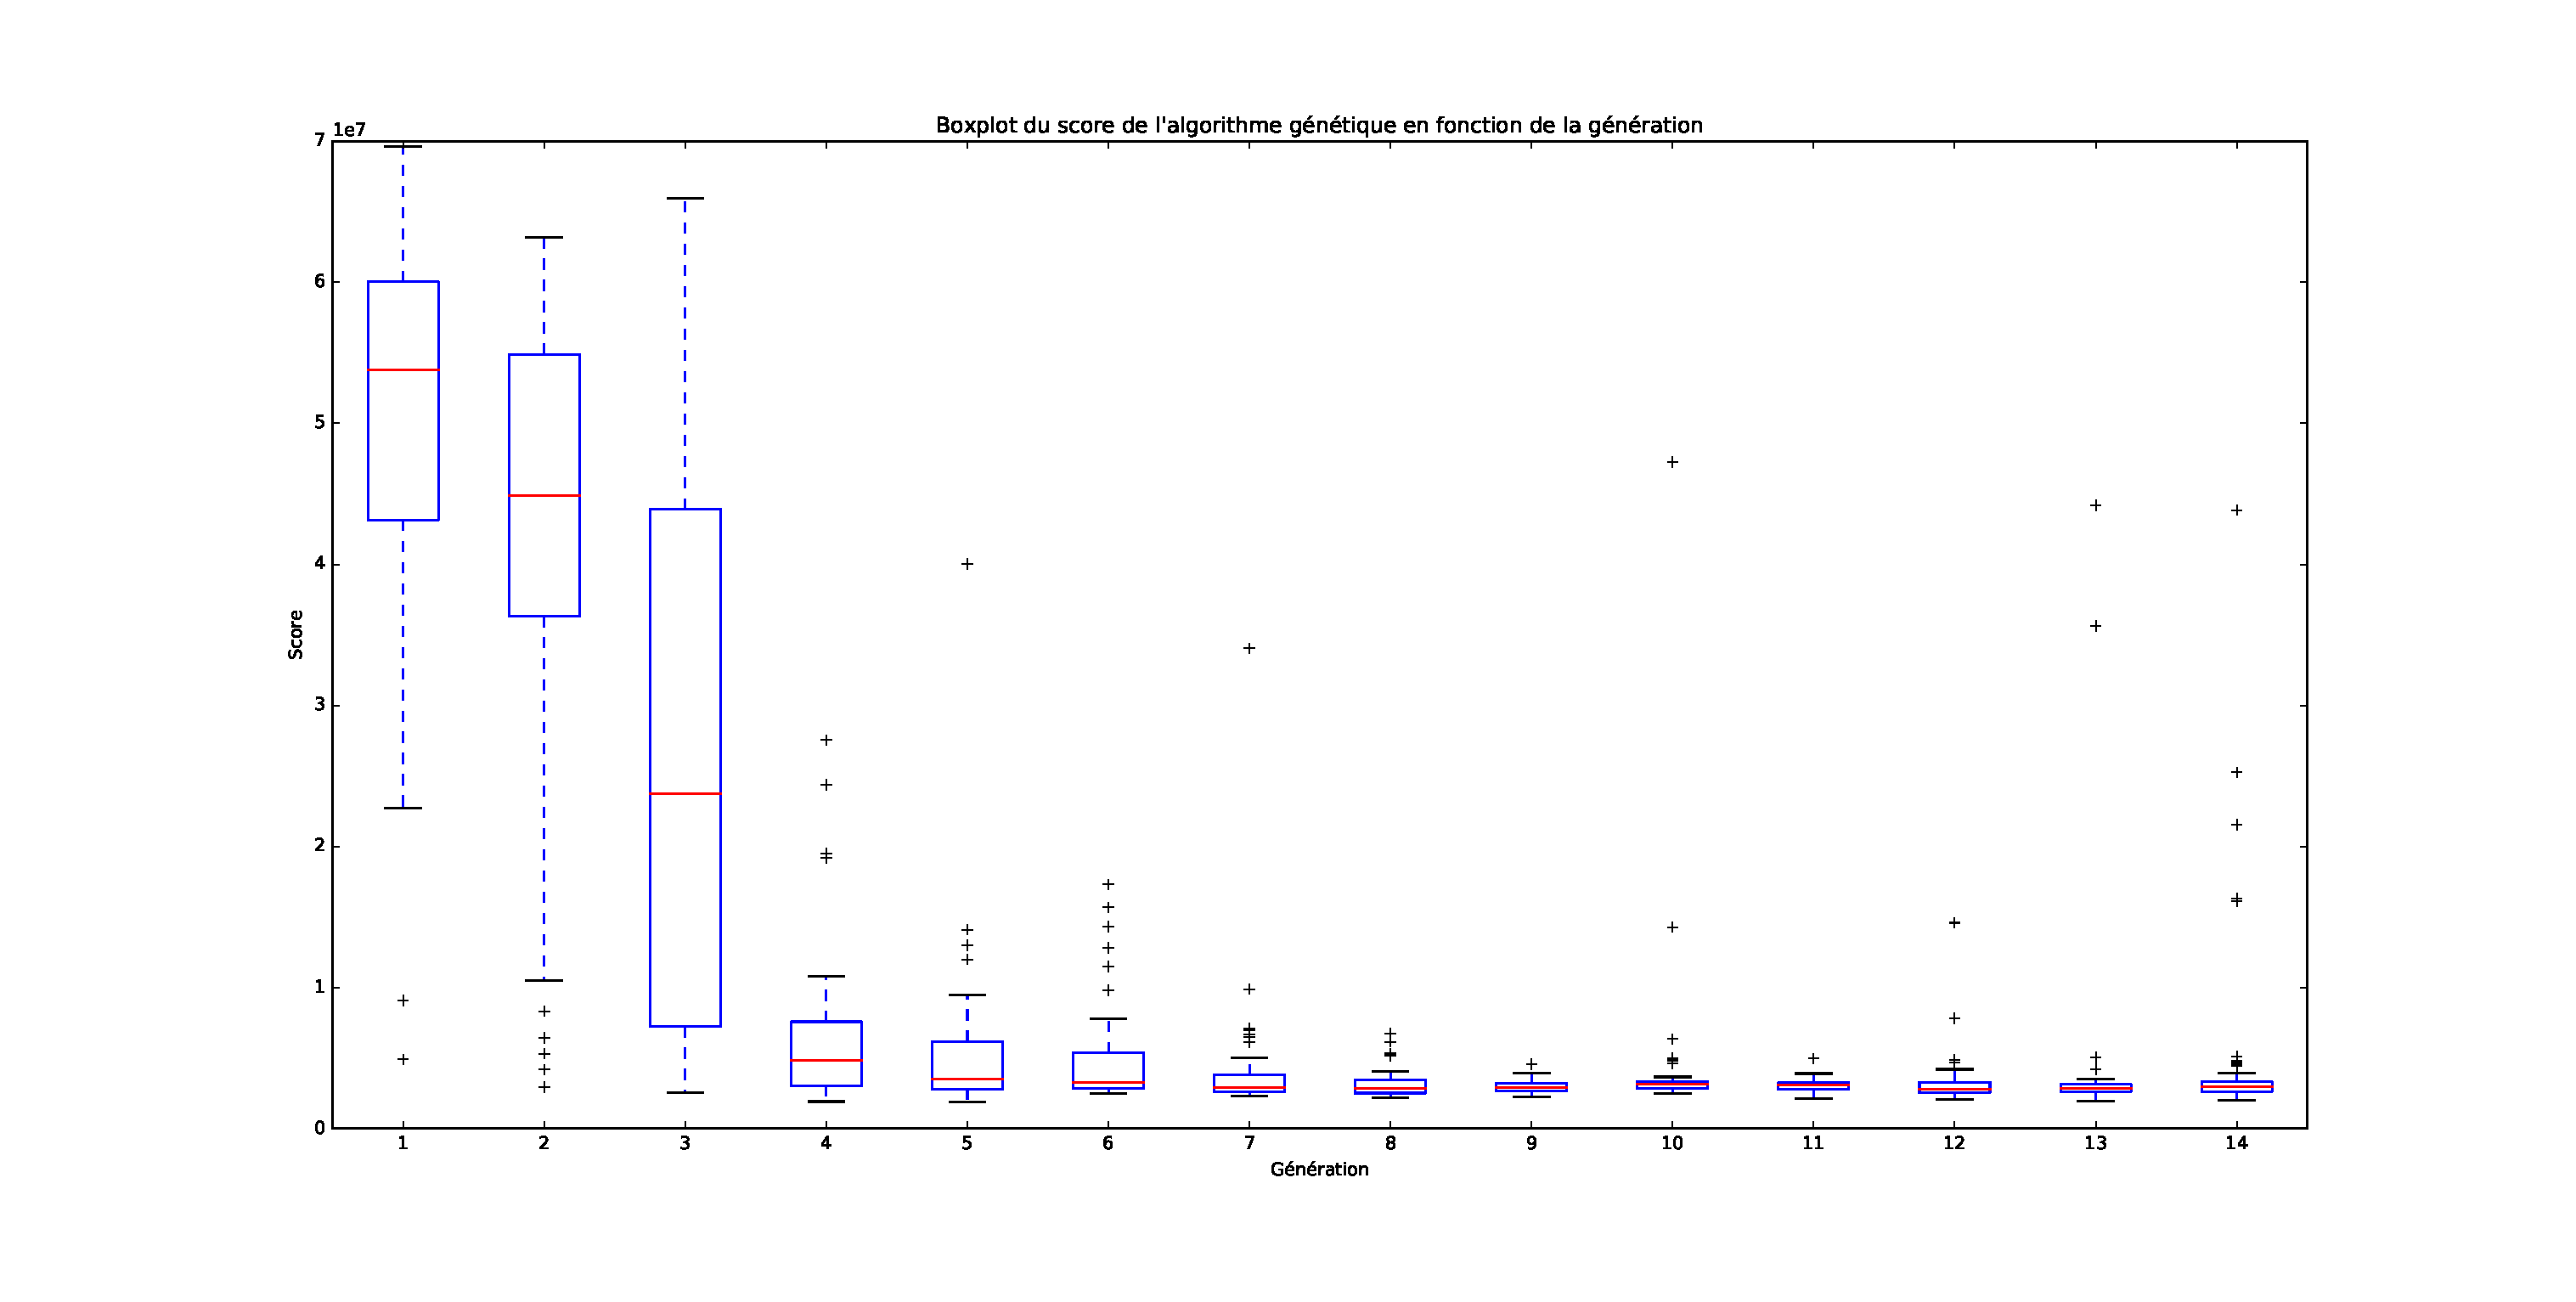
\includegraphics[scale=0.35]{GeneticBoxplot.eps}
    \caption{\label{fig:convergence} Convergence des scores des chromosomes au cours des générations (algorithme génétique)}
\end{figure}

\begin{figure}[htb!]
   \centering
   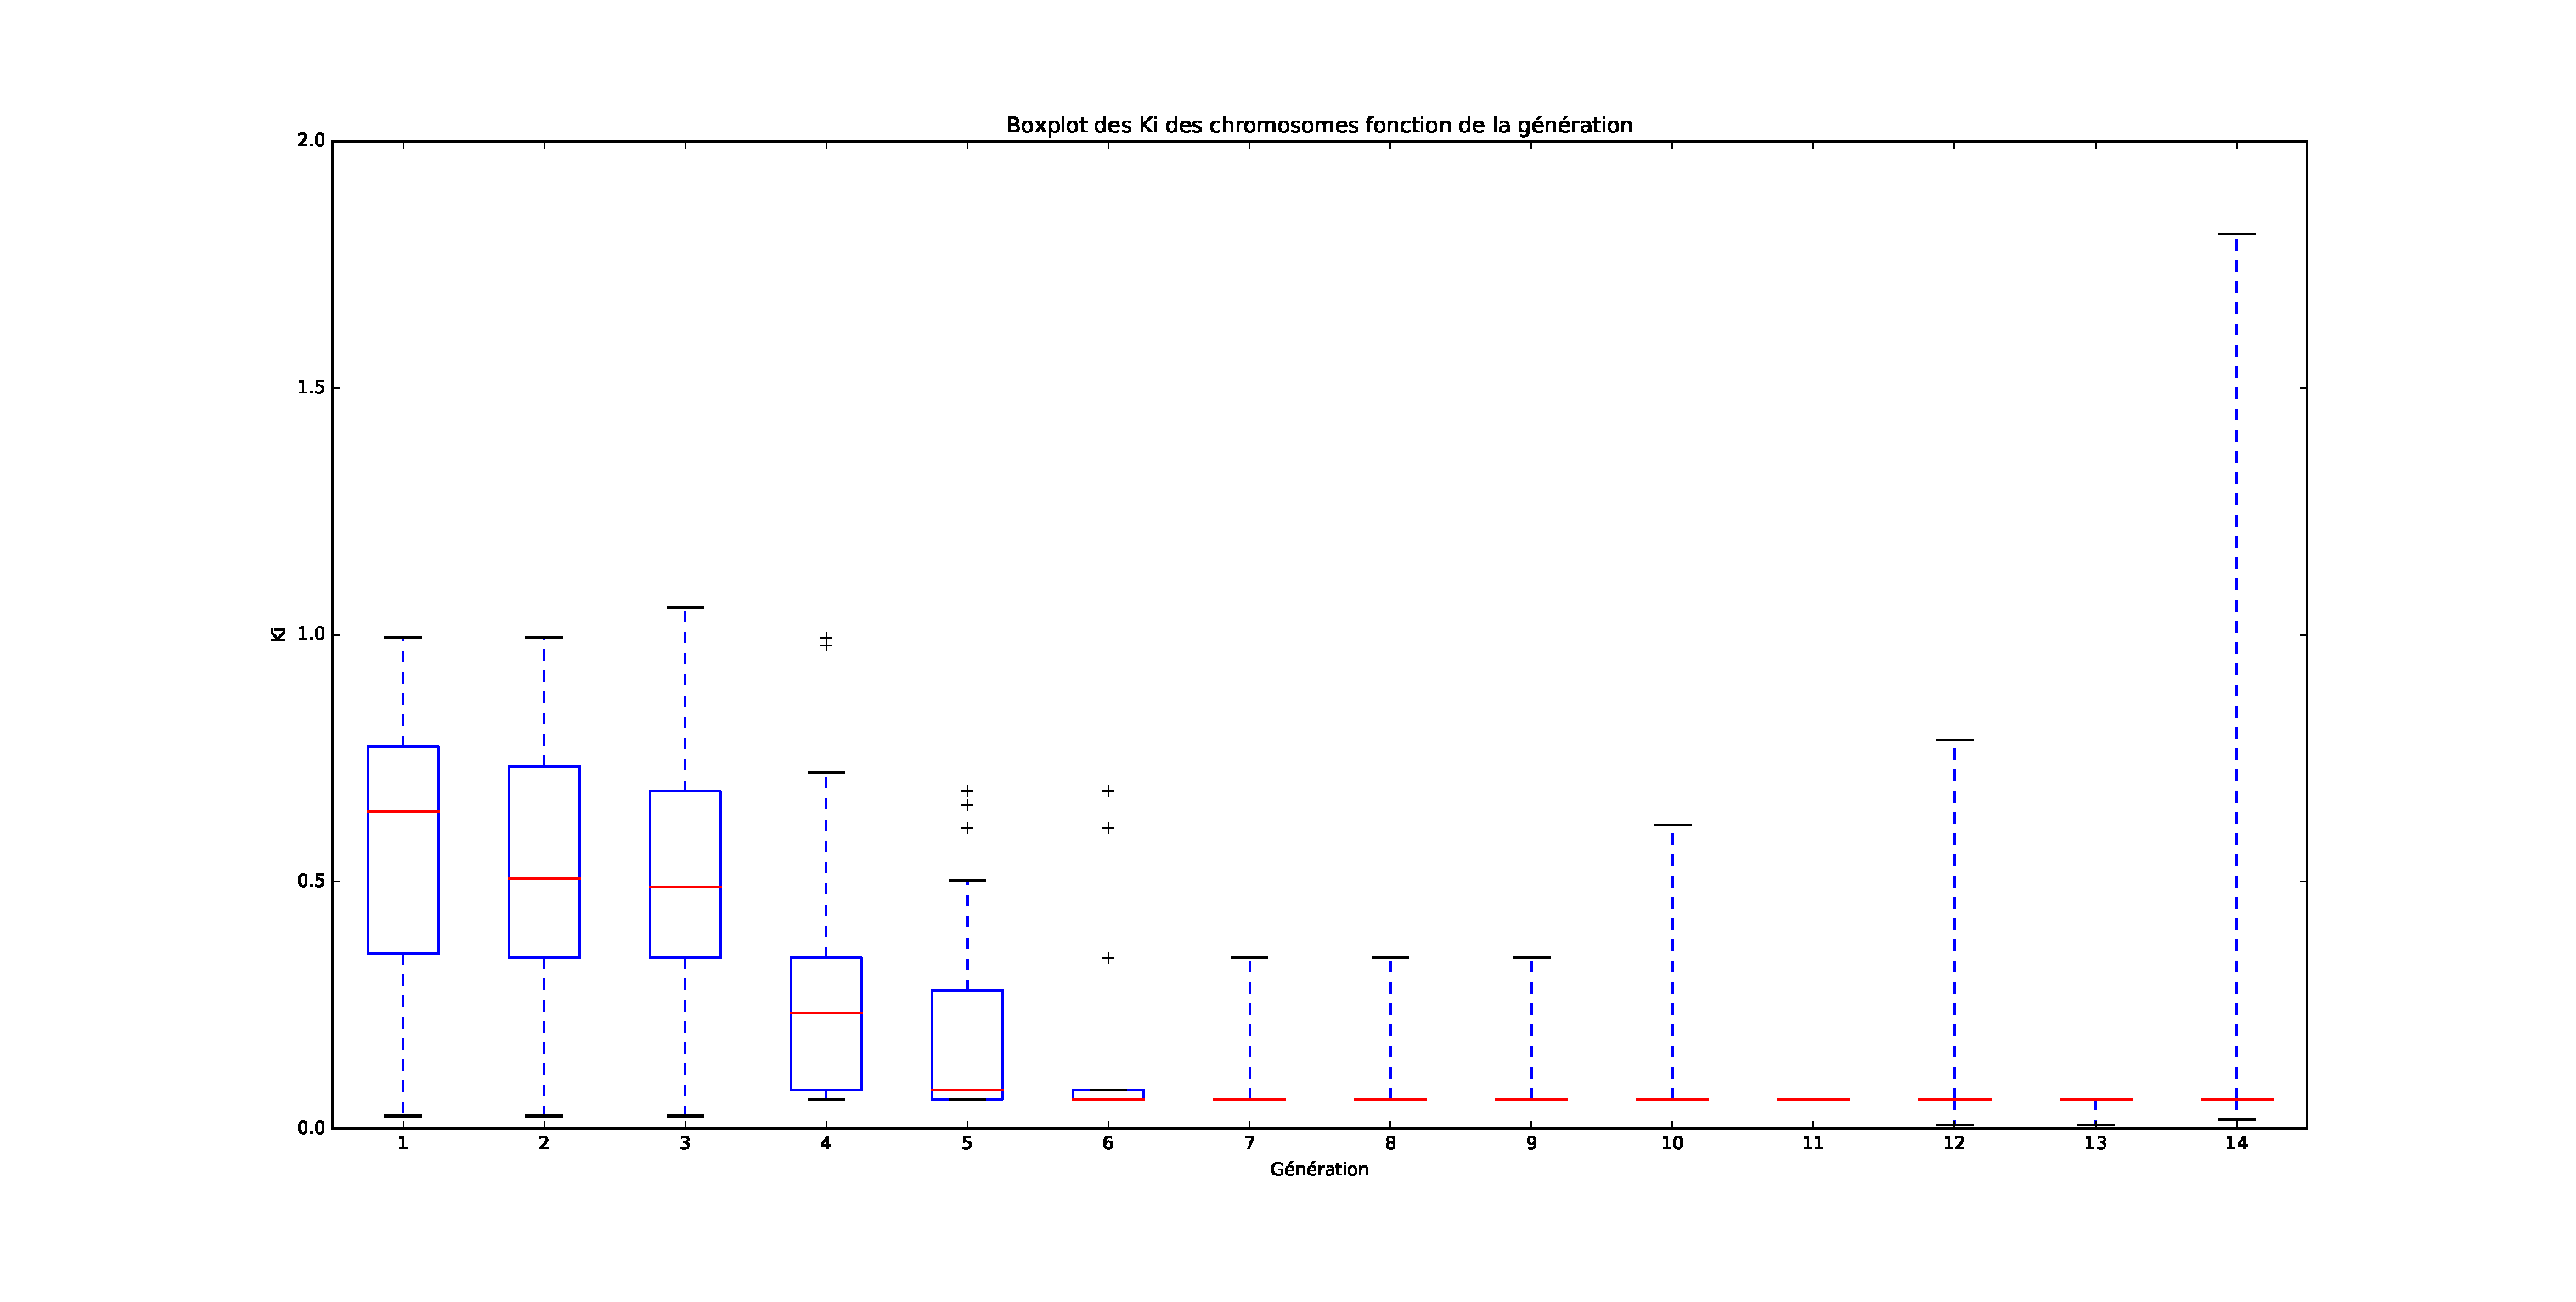
\includegraphics[scale=0.35]{KiBoxplot.eps}
    \caption{\label{fig:kibox} Convergence de $K_i$ des chromosomes au cours des générations.}
\end{figure}


\end{document}
